\documentclass[12pt, twoside]{report}
%% subsection level
\setcounter{secnumdepth}{5}

%% margins, paper size
\usepackage[a4paper,width=150mm,left=30mm,right=30mm,top=24mm,bottom=24mm,bindingoffset=5mm]{geometry}

%% set up the header and footer area
\usepackage{fancyhdr}
\pagestyle{fancy}
\fancyhead{}
\fancyhead[RO,LE]{\thepage}
\fancyhead[LO]{\leftmark}
\fancyhead[RE]{\leftmark}
\fancyfoot{}

%% Make URLs break on hyphens so they don't fall out of page
\usepackage[hyphens]{url}

%% Used to create the box for the abstract
\usepackage{framed}

%% Euro symbol
\usepackage{eurosym}

%% no indentation for paragraphs
\setlength{\parindent}{0pt}

\usepackage[utf8]{inputenc}

%% tables have a bit more space in top and bottom in the rows
\renewcommand{\arraystretch}{1.5}

%% set the graphics path
\usepackage{graphicx}
\graphicspath{ {images/} }

%% for coloring hyperlinks and urls
\usepackage[colorlinks]{hyperref}
\usepackage{breakurl}

%% to change fonts
\usepackage{lmodern}

%% for sub figure captions
\usepackage[font={bf},skip=5pt]{caption}
\usepackage{subcaption}

\renewcommand{\captionlabelfont}{\fontfamily{lmss}}
%% for caption on the side of the image
\usepackage{sidecap}

%% for directory trees
\usepackage{dirtree}

%% multiple column support
\usepackage{multicol}

%% to use colors
\usepackage{xcolor}

%% landscapetomate
\usepackage{pdflscape}

%% draws nice sideways tables
\usepackage{booktabs}
\usepackage{tabularx}
\usepackage[figuresright]{rotating}

%% to make sure that floats don't go to next section
\usepackage{placeins}

%% pages over multiple pages
\usepackage{longtable}

\let\Oldsection\section
\renewcommand{\section}{\FloatBarrier\Oldsection}

\let\Oldsubsection\subsection
\renewcommand{\subsection}{\FloatBarrier\Oldsubsection}

\let\Oldsubsubsection\subsubsection
\renewcommand{\subsubsection}{\FloatBarrier\Oldsubsubsection}

%% js code styles

\definecolor{lightgray}{rgb}{.9,.9,.9}
\definecolor{darkgray}{rgb}{.4,.4,.4}
\definecolor{purple}{rgb}{0.65, 0.12, 0.82}

\usepackage[chapter]{minted}
\usemintedstyle{vs}

\renewcommand{\theFancyVerbLine}{\sffamily {\small \oldstylenums{\arabic{FancyVerbLine}}}}

%% bibliography setup
\bibliographystyle{ieeetr}
\raggedbottom

%% reduce float whitespace
\setcounter{topnumber}{2}
\setcounter{bottomnumber}{2}
\setcounter{totalnumber}{4}
\renewcommand{\topfraction}{0.85}
\renewcommand{\bottomfraction}{0.85}
\renewcommand{\textfraction}{0.15}
\renewcommand{\floatpagefraction}{0.8}
\renewcommand{\textfraction}{0.1}
\setlength{\floatsep}{5pt plus 2pt minus 2pt}
\setlength{\textfloatsep}{5pt plus 2pt minus 2pt}
\setlength{\intextsep}{5pt plus 2pt minus 2pt}

\begin{document}

%% change font to something with less spaces
\fontfamily{lmss}\selectfont

%% preambles
\begin{titlepage}
    \begin{center}
        \vfill

        \large
        \textsc{University of Southampton}
        \\
        {Electronics and Computer Science}

        \vspace{3.0cm}

        \large
        {A group design project report submitted for the award of}\\
        {Master of Engineering}\\

        \vspace{3.0cm}

        by \textbf{GDP 8}:\\
        {Shakib-Bin Hamid}\\
        {Thomas Aley}\\
        {Deepak Thankachan}\\
        {Vlad Catrici}

        \vspace{3.0cm}

        \large
        Project supervisor: Professor Mike Wald\\
        Second examiner: Dr Sepideh Chakaveh\\

        \vspace{3.0cm}

        \textbf{Synote Testing Framework}\\
        \today

        \vfill

    \end{center}
\end{titlepage}

\thispagestyle{plain}

\newgeometry{left=3.67cm,right=3.17cm,top=2.54cm,bottom=2.54cm}

\begin{center}
%    \large
    
    {\fontfamily{ptm}\selectfont

    \textbf{Synote Testing Framework}\\
        
    \vspace{1cm}
    
    \textbf{Group 8} \\
	Shakib-Bin Hamid \\ Thomas Aley \\ Deepak Thankachan \\ Vlad Catrici    
    
    \vspace{2cm}
	}    
\end{center}


%\large
{\fontfamily{ptm}\selectfont
\textbf{Supervisor}: Professor Mike Wald\\
\textbf{2nd Examiner}: Dr Sepideh Chakaveh\\
\textbf{Customer}: Synote Limited (Professor Mike Wald and Dr Yunjia Li) 12 Merlin Way, Eastleigh, SO53 4JB
}

\vspace{1cm}

\begin{framed}

{\fontfamily{ptm}\selectfont
Abstract\\

Synote, a company derived from previous successful projects at the University of Southampton, provides automated transcripts for uploaded videos. However, it required a payment system. It was also ineffective in its previous efforts to build an End-to-End (E2E) testing framework and did not have a Continuous Integration (CI) process in place. All three are mission critical for any successful software company. Initially, GDP team 8 set out to deliver the former two. At the same time, they achieved $\approx$ 100\% test coverage in their implementation using unit, integration and E2E tests. Near the end, the team focused on implementing a CI process for Synote as an extension to the project. Overall the group delivered a secure payment system, a practical E2E testing framework with comprehensive tests and a CI implementation for the experiment stage of deployment. They also provided the E2E testing methodology and the QA process as a document. This report will cover the details of each of the deliverables, as well as the team management and future works of the project.
}
\end{framed}

\restoregeometry


\chapter*{Declaration}
We are aware of the requirements of good academic practice and the potential penalties for any breaches. We confirm that this project report and the accompanying code are all our own work except the open-source frameworks and libraries, which are referenced and credited in the report and code.
\chapter*{Acknowledgements}


%% content list
\tableofcontents
\listoffigures
\listoftables
\listoflistings

%% main body
\chapter{Introduction}
\label{chap:introduction}

\section{Location of files}
\label{sec:location-files}
Chapters go in \texttt{chapters} folder. Figures in \texttt{images} folder. No content must be written elsewhere. All content must lie in chapters files'. We may need to create files for sections, if chapters get too big.

\section{Writing Content}
\label{sec:content}
You must not write live on Overleaf! I cannot emphasize it enough! Download the project as a git repo from the options on overleaf. Then write what you need to write, compile locally, then once everything compiles nice and well, put it on overleaf.

\section{Formatting}
\label{sec:formatting}

End each paragraph with a double backslash always.\\

\subsection{Labeling}
\label{subsec:labeling}
Make sure you label 'every component' with a label like above. Chapters will have labels as \texttt{chap:name}, sections as \texttt{sec:name} and so on.

\subsubsection{Naming labels}
\label{subsubsec:naming-labels}
Use all small alphabets in labels, separated by dash (-).\\

This way we can refer any Chapter, Section, Table, Figure, sub components etc.

\subsection{Referring Components}
\label{subsec:referring-components}

You should do bold-face for reference as follows -

\textbf{Section \ref{subsubsec:naming-labels}} is about how to name labels and \textbf{Chapter \ref{chap:introduction}} is the introduction.

\subsection{Figures}

You should place the figures in the \texttt{figures} folder. They should be transparent background in most cases, named all lower cases with dashes. You must label them as \texttt{fig:name}\\

\begin{figure}[!hbt]
  	\centering
 	
\includegraphics[width=0.3\textwidth]{exm.jpg}
  	\caption{Normal figure}
 	\label{fig:normal-figure}
\end{figure}

All figures must have captions as well. Sub figures may be left caption less, as long as the entire figure has caption.\\

You can use minipage to insert subfigures as done in \textbf{Figure \ref{fig:subfig-minipage}}. This is the recommended way. Otherwise you can use \textbf{Figure \ref{fig:right-side-minipage}}\\

\begin{figure}[!htb]
    \centering
    \begin{minipage}{.5\textwidth}
        \centering
        
\includegraphics[width=0.25\textheight]{exm.jpg}
        \caption{Left side image}
        \label{fig:left side minipage}
    \end{minipage}%
    \begin{minipage}{0.5\textwidth}
        \centering
        
\includegraphics[width=0.25\textheight]{exm.jpg}
        \caption{Right side image}
        \label{fig:right-side-minipage}
    \end{minipage}
    \caption{Subfigures using minipage}
    \label{fig:subfig-minipage}
\end{figure}

The subfigure package has caused me problems before, I suggest against it. Similarly, you can use \textbf{Figure \ref{fig:sidecaption-fig}} to have side by side caption or text. You can refer to subfigures as well like \textbf{Figure \ref{fig:left-side-image}} I suggest against it. Use two minipages - one side normal figure, other side text for the figure.

\begin{figure}[!hbt]
    \centering
    \begin{subfigure}[b]{0.4\textwidth}
        
\includegraphics[width=\textwidth]{exm.jpg}
        \caption{Left side image}
        \label{fig:left-side-image}
    \end{subfigure}
    ~ %add desired spacing between images, e. g. ~, \quad, \qquad, \hfill etc.
      %(or a blank line to force the subfigure onto a new line)
    \begin{subfigure}[b]{0.4\textwidth}
        
\includegraphics[width=\textwidth]{exm.jpg}
        \caption{Right Side Image}
        \label{fig:right-side-image}
    \end{subfigure}
    \caption{Side by side figures using subfigures}
    \label{fig:subfigure}
\end{figure}

\begin{SCfigure}
  \centering
  \caption{Side label with possibly a large amount of text. This is how you would write it}
  
\includegraphics[width=0.3\textwidth]{exm.jpg}% filename
  \label{fig:sidecaption-fig}
\end{SCfigure}

\section{Adding Tables}
\label{sec:adding-tables}

Tables must be labeled with usual labeling convention. Also the use of \texttt{multicol} package allows for centering text in table fields and merging of fields as shown in the example below.

Referring to a table example: As show in \textbf{Table \ref{tab:myTable}}. \\

%Column widths dependent on page width/margins
\begin{tabular}{ |p{0.5cm}|p{4cm}|p{4cm}|p{4cm}|  }

 \hline
 	%Example of column merging
 	\multicolumn{4}{|c|}{Table Title Example} \\
 \hline
 	%Examples of centering text
 	\multicolumn{1}{|c|}{id} &
 	\multicolumn{1}{|c|}{Column Heading} &
 	\multicolumn{1}{|c|}{Column Heading} &
 	\multicolumn{1}{|c|}{Column Heading}  \\
 \hline
 	1 & Field 1,1 & Field 1,2 & Field 1,3 \\
 \hline
 	2 & Field 2,1 & Field 2,2 & Field 2,3 \\
 \hline
 	3 & Field 3,1 & Field 3,2 & Field 3,3 \\
 \hline

\end{tabular}
%Use of captionof allows 'Table' instead of default 'Figure'
\captionof{table}{My Table Example}
\label{tab:myTable}
\vspace{0.4cm}

When a larger table is needed that would fit better on a landscape page, the \texttt{rotating} package can be used and a \texttt{sidewaystable} defined as shown in the example on the next page: \textbf{Table \ref{tab:mySidewaysTable}}.

\begin{sidewaystable}
  \begin{tabular}{ |p{0.5cm}|p{7cm}|p{7cm}|p{7cm}|  }
    \hline
        \multicolumn{4}{|c|}{Sideways Table Title Example} \\
     \hline
        \multicolumn{1}{|c|}{id} &
        \multicolumn{1}{|c|}{Column Heading} &
        \multicolumn{1}{|c|}{Column Heading} &
        \multicolumn{1}{|c|}{Column Heading}  \\
     \hline
        1 & Field 1,1 & Field 1,2 & Field 1,3 \\
     \hline
        2 & Field 2,1 & Field 2,2 & Field 2,3 \\
     \hline
        3 & Field 3,1 & Field 3,2 & Field 3,3 \\
     \hline

  \end{tabular}
  \captionof{table}{My Sideways Table Example}
  \label{tab:mySidewaysTable}
\end{sidewaystable}


\section{Code Listing}
\label{sec:code-listing}

You can add code snippets as seen in \textbf{Listing \ref{lst:listing-main}} or \textbf{Listing \ref{lst:side-listing}} full width or mini page listing.

\begin{minipage}{.5\textwidth}
  \begin{listing}[H]
  \begin{minted}[xleftmargin=\parindent, linenos, breaklines, breakanywhere, bgcolor=lightgray, fontsize=\small]{js}

  Name.prototype = {
    methodName: function(params){
      var doubleQuoteString = "some text";
      var singleQuoteString = 'some more text';
      // this is a comment
      if(this.confirmed != null && typeof(this.confirmed) == Boolean && this.confirmed == true){
        document.createElement('h3');
        $('#system').append("This looks great");
        return false;
      } else {
        throw new Error;
      }
    }
  }

  \end{minted}
  \captionof{listing}{caption}
  \label{lst:label-for-listing}
  \end{listing}
\end{minipage}%
\begin{minipage}{0.5\textwidth}
	\centering
	
\includegraphics[width=0.25\textheight]{exm.jpg}
	\caption{Right side image}
	\label{fig:right-side-minipage}
\end{minipage}

\begin{listing}[H]
\begin{minted}[xleftmargin=\parindent, linenos, breaklines, breakanywhere, bgcolor=lightgray, fontsize=\small]{js}

Name.prototype = {
  methodName: function(params){
    var doubleQuoteString = "some text";
    var singleQuoteString = 'some more text';
    // this is a comment
    if(this.confirmed != null && typeof(this.confirmed) == Boolean && this.confirmed == true){
      document.createElement('h3');
      $('#system').append("This looks great");
      return false;
    } else {
      throw new Error;
    }
  }
}

\end{minted}
\captionof{listing}{caption}
\label{lst:label-for-listing}
\end{listing}

\section{References}
References are written in \texttt{references.bib} file. I will demo you personally about how to write references. Each reference has a key and you can refer it like this \cite{iansommerville2011}.\\


\section{Directory Trees}
\label{sec:dir-trees}

Directory trees are nice and simple using the package \texttt{dirtree} as shown below in \textbf{Figure \ref{fig:dir-tree}}.

\dirtree{%
  .1 Directory.
  .2 Folder 1.
  .3 Sub Folder 1.
  .4 File 1.
  .2 Folder 2.
}
\captionof{figure}{Directory Tree Example}
\label{fig:dir-tree}

\chapter{Project Management}
\label{chap:project-management}

Project management is often left as a side topic in university projects. Sadly, this practise often results in either the project not achieving its true potential, or in worst cases catastrophic failure. It may be because of poor time management, risks for an unprepared team, a dominating project manager or the simple lack of teamwork. We believe that a Group Design Project (GDP) should have at least the following as their project management goals \cite{iansommerville2011}:

\begin{itemize}

  \item Timely delivery to the customer
  \item Meeting the customer's expectations
  \item Maintain a well-functioning development team

\end{itemize}

Shakib was the project manager for GDP 8. We are proud of the professionalism that we have demonstrated during the project. We were pragmatic in our time management, professional and honest in our communication with our supervisor and our client and finally we managed our risks well. In this chapter we will analyse how we were able to achieve the above goals.

\section{Risk Analysis}
\label{sec:risk-analysis}

We will begin with risk analysis, since our management techniques evolved through our efforts in mitigating the major risks. In \textbf{Table \ref{tab:risk}} we list the \textit{major} risks - those that clearly affect the project and the products we produced. In the following sections we discuss how we managed the risks and in turn managed our project.

\pagebreak

\begin{center}

\begin{longtable}{ |p{6cm}|p{1.9cm}|p{2.2cm}|p{2.6cm}| }

 \hline
 	%Example of column merging
 	\multicolumn{4}{|c|}{Risk Analysis} \\
  \hline
  	\multicolumn{1}{|c|}{Risk} &
  	\multicolumn{1}{|c|}{Affects} &
  	\multicolumn{1}{|c|}{Probability} &
  	\multicolumn{1}{|c|}{Effect}  \\
  \hline
 	 Goals are not clear & Project, Product & Very High & Catastrophic \\
   \hline
   Software not to specification & Product & Very High & Catastrophic \\
   \hline
   Changing requirements & Project, Product & High & Serious \\
  \hline
  Team member unavailable/left & Project & Very High & Serious \\
  \hline
  Technologies unavilable e.g. VM & Product & Very High & Serious \\
  \hline
  Under-performing software & Product & Low & Tolerable \\
  \hline
  Payment system faulty & Product & Very Low & Catastrophic \\
  \hline
  Continuous integration faulty & Product & Very Low & Tolerable \\
  \hline
  \caption{Risk Analysis}
  \label{tab:risk}
\end{longtable}

\end{center}
\vspace{-1cm}

\section{Time Management}
\label{sec:time-management}
Since a 4th year MEng student should spend 2/3 of their time on the GDP, we estimated that we should each spend at least 30 hours/week (out of 50 hours/week) on our project. In our previous experience we found it very difficult to keep to strict hours because of other commitments e.g. societies, coursework etc.\\

To mitigate this risk, we booked a library room \textit{every weekday} for the entire 1st semester. This ensured that we always had a place to work together. We insisted on maximising our contact time. In fact we utilised the room bookings to the fullest extent by working above \textit{\textbf{30 hours}} together each week (\textbf{Appendix \ref{appendix:team-member-contribution}}).\\

We also estimated the work amount for other coursework in advance and worked more on our GDP in certain weeks. We kept our supervisor and our client well informed of our commitments each week so that we could prepare thusly. Our Gantt Chart in \textbf{Appendix \ref{appendix:gantt-charts}} illustrates that we followed our original plan well since work hours closely match our initial estimates. In fact, the only change is that we finished our initial goals earlier than anticipated and could focus on further achievements like CI.

\section{Weekly Meetings}
\label{sec:weekly-meetings}
We met both the supervisor and the client at least once each week since the start of the term. The goals of the meetings were to:

\begin{itemize}

  \item Demonstrate the current progress
  \item Prioritise tasks for the following week
  \item Ensure that the client is satisfied with the direction and progress

\end{itemize}

These meetings mitigated the risk of not achieving the specification and guarded us from veering off course.\\

A key focus during these meetings was to clarify project goals, deliverables and the success criteria. This made us confident in our progress each week, since we could justify our project direction during demonstrations, based on the agreed objectives from the previous meetings. We tried to be as empirical as possible in estimating our work during the meetings so that we neither over-estimated, nor under-estimated the difficulty. Not only did this help us achieve our initial goals, but it also helped us extend the deliverables to implement Synote's first successful attempt at CI.\\

We met our client at least once more each week in addition to regular contact over \textit{Slack}. This ensured that we were following his coding conventions and greatly helped when we merged our code each week.

\section{Team Management}
\label{sec:people-management}
Our project manager, Shakib, focused on the following to manage the team \cite{iansommerville2011}:

\begin{itemize}

  \item Team members gain new skills
  \item Each member feels included in the project
  \item Each member is treated identically
  \item Honesty about the team's progress and individual contributions

\end{itemize}

The following sections better explain how the team managed the skills and tasks among themselves.

\subsection{Dividing Work}
\label{subsec:dividing-work}
We started a weekly team meeting after the first progress seminar feedback from the supervisor. During this meeting we set our personal weekly tasks. Previously task assignment was done informally.\\

Usually after the weekly meeting (\textbf{Section \ref{sec:weekly-meetings}}), we had 4-5 different major tasks for the week. The team members that were present during the team meetings picked the tasks they preferred. Otherwise, the manager assigned a task if any member was absent or did not have a preference. Finally he picked the remaining tasks.\\

If a team member finished his own tasks early, he helped out with others' remaining tasks. Similarly, if one's task depended on another's and it was blocking the former's progress, they would either collaborate, or continue the other's work while they may be absent. Every effort was made to ensure that each developer had a task.\\

\textbf{Appendix \ref{appendix:team-member-contribution}} clearly indicates each team member's individual contribution to the project. \textbf{Appendix \ref{appendix:code-commits}} is the evidence in terms of code commits that they  produced. For example Shakib performed nearly 60\% of the tasks of Synote's CI set up, Vlad and Tom each did 20\% of the tasks in CI, while Deepak wrote nearly 70\% of the E2E test cases of payment feature.\\

It must be noted though - not all contribution can be measured in terms of code line commits alone, since there were significant tasks that could not be committed as code - research for example, or when collaborated code was committed from a single user. So, we have included further diagrams to clarify when a team member contributed to the project in the following sections.

\subsection{Collaboration}
\label{subsec:collaboration}

Even though we each had our personal tasks that we completed every week (as explained in \textbf{Section \ref{subsec:dividing-work}}), 25 - 30\% of our tasks  required joint effort. Similar to any well functioning software development group, we often divided our work and came together to combine our efforts to achieve a requirement.\\

\textbf{Appendix \ref{appendix:team-collaboration}} clearly shows the timelines of each team member's major tasks throughout the project and illustrates where and when he collaborated with others.\\

\begin{figure}[!hbt]
  	\centering
 	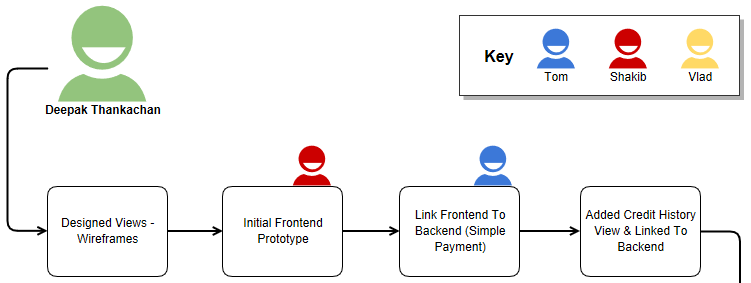
\includegraphics[width=0.8\textwidth]{deepak-collab-snip.png}
  	\caption{Example of collaboration diagram}
 	\label{fig:deepak-collaboration-snippet}
\end{figure}

For example from \textbf{Figure \ref{fig:deepak-collaboration-snippet}}, which itself is a snippet from the appendix, we know that Deepak worked with Tom to integrate the initial server side REST API for the payment feature with his client side implementation.

\subsection{Team Skills}
\label{subsec:team-skills}

A major concern was the team's lack of practical JavaScript knowledge, especially when the entire Synote application is JavaScript based. Shakib was the most proficient in JavaScript and he worked with each team member to help them with JavaScript to mitigate the risk early. The rest of the team worked hard in the first 4-5 weeks to overcome any technical difficulties, including learning promise based structures, dynamic typing, closures and the frameworks: Sails, Angular JS, Protractor, Cucumber etc.\\

The team has picked up a number of development skills after this project. Tom and Vlad are more confident in their JavaScript knowledge, Deepak is more fluent in front end development in Angular JS and HTML 5 than ever before and finally Shakib is assured of his JavaScript, Linux and team management skills. Each team member also learned a significant amount about the proper use of version control (\textbf{Section \ref{sec:code-submission-process}}). The team members are also more optimistic about their individual strengths, as well as the group synergy.

\subsection{Team Inclusion and Honesty}
\label{subsec:team-inclusion}
The manager, Shakib, emphasised equality and inclusion of team members in their contribution to the project. Each member was informed of the other's contributions through a shared document (\textbf{Appendix \ref{appendix:team-member-contribution}}). He also informed absent team members about group decisions after each meeting so that they felt included. Any discrepancy was openly discussed with the team member so that they felt equally valued and no one wast left with unfair resentment.\\

Similarly all team members respected each other's responsibilities and even contributed to alleviate other's issues, for example: fill in the hours if someone was unavailable due to a job interview.

\section{Code Quality Management}
\label{sec:code-quality-management}

We had the following goals for our JavaScript coding style and quality:

\begin{itemize}

  \item Follow the industry's best practices
  \item Follow the existing practices in Synote's codebase
  \item All code must be reviewed by at least one other team member

\end{itemize}

We followed the conventions of Synote's lead developer to ensure that the client can easily add further functionality. In fact, we documented the conventions we followed in the \texttt{CONTRIBUTING.md} document for Synote so that the future developers also follow the same conventions.\\

As discussed before, code produced during pair programming was continuously reviewed by both team members. Similarly Shakib reviewed all code written by the team members before submitting it to the client each week. Static checks to find common JavaScript issues that may indicate bugs (e.g. undeclared/unused variables) were also marked by 'linters' provided in the IDEs. We also achieved almost complete test coverage in the payment feature through server side unit/integration and E2E tests (\textbf{Appendix \ref{appendix:server-test-cases}} and \textbf{\ref{appendix:e2e-testing}}). Finally, the client also provided feedback about the code we submitted and we refactored accordingly, for example: use of services on the client side, promises throughout the application etc.

\section{Code Submission Process}
\label{sec:code-submission-process}

We had the following goals in terms of code submissions:

\begin{itemize}

  \item Submit code to the client weekly
  \item Commit often
  \item Review often
  \item Reduce merge conflicts

\end{itemize}

In order to achieve the goals, we adopted a code submission strategy (\textbf{Figure \ref{fig:version-control}}). Shakib forked both the client's E2E testing and application repositories to create GDP8 repositories. The master branch of the GDP8 repositories were regarded stable and no direct commits were made on the master branches. Instead we created feature branches from the GDP8 master branches and each developer submitted code to the feature branch every day. At the end of the day, there would be no work left to be submitted to the feature branch.\\

\begin{figure}[!hbt]
  	\centering
 	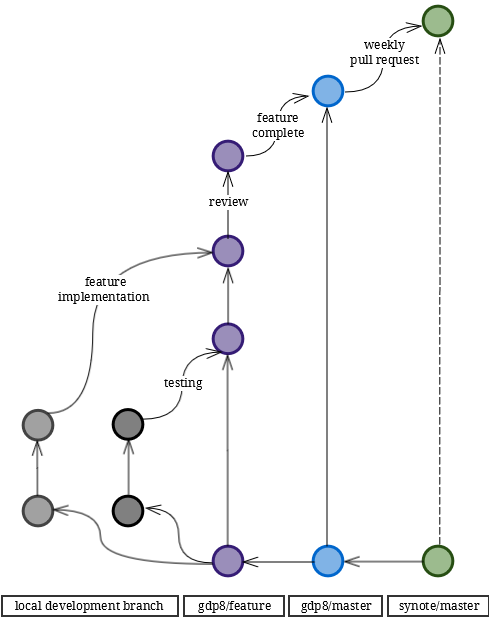
\includegraphics[width=0.8\textwidth]{commits.png}
  	\caption{Version Control}
 	\label{fig:version-control}
\end{figure}

Once a feature was nearly complete, code review was performed on the feature branches. On Fridays, Shakib pushed the stable code to GDP8 master branches, merged with the latest client's master branch and finally re-ran all the tests. This ensured that the client had minimal effort in merging our one week's worth of code. In fact, we had \textbf{\textit{no conflicts}} in submitting our code to the client and did not break any functionality on the client's existing repositories, even when there were multiple other groups working on them.

\chapter{Background Reading}
\label{chap:background-reading}
\chapter{Payment Feature}
\label{chap:payment-feature}

% Nomenclature - JSON?

\section{Sever Side Implementation}
\label{sec:server-side-implementation}

The greatest concern in implementing a payment feature for Synote is remaining PCI DSS (Payment Card Industry Data Security Standard) compliant. To remove most of the burden and with the approval of our client Yunjia Li, Stripe was chosen as the payment gateway. Stripe also allows custom merchant forms which our client favours over redirection and generated forms.\\

\begin{figure}[!hbt]
  	\centering
 	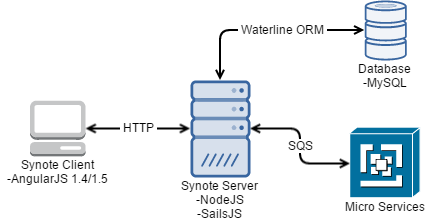
\includegraphics[width=0.78\textwidth]{synote-architecture.png}
  	\caption{Synote Architecture}
 	\label{fig:synote-architecture}
\end{figure}

\textbf{Figure \ref{fig:synote-architecture}} depicts Synote's existing architecture which uses Node.js (Node) and Sails.js (Sails) web frameworks on the server. Sails includes a powerful Object Relational Mapping (ORM) tool called Waterline to provide a data access layer to the underlying MySQL database.\\

As a custom merchant form is desired for gathering payment information, Stripe must be used to tokenize the payment data before it can be sent to Synote's server. As mentioned in \textbf{Section \ref{subsec:security}}, HTTPS is required for secure transmission of payment data over a network, so the first stage of integration is to use an HTTPS/SSL certificate to enable HTTPS communication. The resulting architecture is shown in \textbf{Figure \ref{fig:stripe-integration}}.\\

\begin{figure}[!hbt]
  	\centering
 	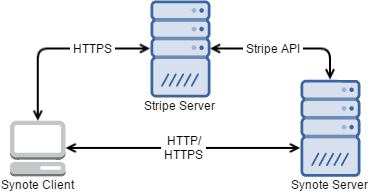
\includegraphics[width=0.7\textwidth]{stripe-integration.png}
  	\caption{Integrating Stripe}
 	\label{fig:stripe-integration}
\end{figure}

The first iteration of the payment feature requires simple functionality: A customer must be able to enter payment information to buy \texttt{X} amount of credits which will be stored against their Synote account, along with a record of the transaction. \textbf{Figure \ref{fig:simple-sequence}} shows the full sequence of events necessary to achieve this behavior, however, server side implementation concerns only what happens as a result of the \texttt{POST} action to Synote's server.\\

\begin{figure}[!hbt]
  	\centering
 	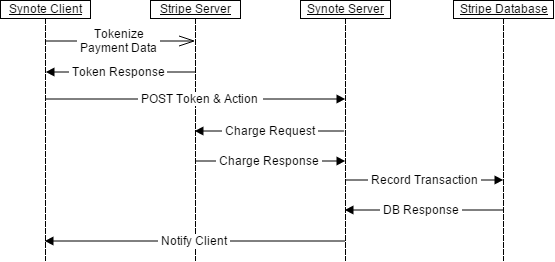
\includegraphics[width=\textwidth]{simple-sequence.png}
  	\caption{Sequence Diagram Of Simple Payment}
 	\label{fig:simple-sequence}
\end{figure}

Step one is to create the endpoint to which a Stripe token and any additional required information can be posted. Sails has an API called Blueprint which creates RESTful routes when an endp oint is created with a \texttt{model} and \texttt{controller}. Further routes can be added to the endpoint route through the concept of action routes, thus a \texttt{controller} file named \texttt{CreditHistoryController.js} containing an action route of \texttt{topup} exposes the route: \texttt{/credithistory/topup}.\\

Making charges against a token requires Stripe's API \cite{stripe-api} which can be added using the \texttt{require} keyword and must include a secret key provided by Stripe. Stripe's API lists examples of functions in Node, but in the form of callbacks. As covered in \textbf{Section \ref{sec:synote}}, the convention is to use promises in favour of callbacks which altogether results in code similar to \textbf{Listing \ref{lst:stripe-charge}}.\\

\hspace{0.1\textwidth}
\begin{minipage}{.76\textwidth}

\begin{listing}[H]
\begin{minted}[xleftmargin=\parindent, linenos, breaklines, breakanywhere, bgcolor=lightgray]{js}
return stripe.charges.create({
        amount: cost,
        currency: "gbp",
        source: token.id
});
\end{minted}
\captionof{listing}{Stripe Charge Promisified Example}
\label{lst:stripe-charge}
\end{listing}
\end{minipage}
\hspace{0.1\textwidth}
\vspace{0.3cm}

Information required to make a charge includes a single use token, charge amount and currency. The token and charge amount are provided in the \texttt{POST} from a client as a JSON object in the request (\texttt{req}) body. It is convention that a \texttt{req} is only processed within a \texttt{policy} and \texttt{controller}. Sails uses policies for authorization and access control such that each \texttt{action route} for each \texttt{controller} can be assigned one or more policies. As Synote uses Auth0 \cite{auth0} a policy called \texttt{hasJsonWebToken} exists to add a user's profile to a \texttt{req} which, aside from authorization, has the added benefit of providing a user's ID that can be used to determine which user is making a purchase.\\

\begin{figure}[!hbt]
  	\centering
 	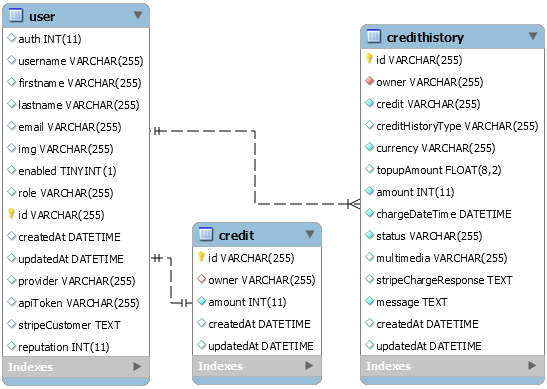
\includegraphics[width=\textwidth]{db-credit.png}
  	\caption{Credit \& Credit History Database Tables}
 	\label{fig:db-credit}
\end{figure}

The remaining task is recording the transaction and assigning purchased credits to a user. The setup for this task requires alteration to the existing database (DB), a Sails \texttt{model} and Waterline methods to interact with the DB. \textbf{Figure \ref{fig:db-credit}} shows the schema of the credit and credit history tables with their relations to the existing user table. Adding these tables to an existing database requires use of an SQL migration file as shown in \textbf{Listing \ref{lst:migration-file}}.\\

\hspace{0.1\textwidth}
\begin{minipage}{.72\textwidth}
\begin{listing}[H]
\begin{minted}[xleftmargin=\parindent, linenos, breaklines, breakanywhere, bgcolor=lightgray, fontsize=\small]{sql}
DROP TABLE IF EXISTS `testing`;
CREATE TABLE `testing` (
  `id` VARCHAR(255) NOT NULL,
  `email` VARCHAR(255) NOT NULL,
  `role` VARCHAR(255) NOT NULL,
  `free` BOOLEAN DEFAULT TRUE,
  `createdAt` datetime DEFAULT NULL,
  `updatedAt` datetime DEFAULT NULL,
  PRIMARY KEY (`id`)
) ENGINE=InnoDB DEFAULT CHARSET=utf8;

\end{minted}
\captionof{listing}{Section Of Migration File: v0.9.0-v0.10.0.sql}
\label{lst:migration-file}
\end{listing}
\end{minipage}
\hspace{0.1\textwidth}
\vspace{0.3cm}

A section of the \texttt{model} file required for Waterline ORM to interact with the database is shown in \textbf{Listing \ref{lst:credit-history-model}}. Each attribute of the \texttt{model} is a one-to-one mapping with a field in the corresponding table, in this case \texttt{stripeChargeResponse} is shown with a type of \texttt{text} which can clearly be seen in the \texttt{credithistory} table of \textbf{Figure \ref{fig:db-credit}}. This field exists to store a record of the charge response from Stripe and contains redacted PCI DSS compliant information such as the last four digits of the charged card. Also of note in \textbf{Listing \ref{lst:credit-history-model}} are two examples of Waterline functions: \texttt{findOne} and \texttt{update} which in this instance are part of a hook to update the quantity of credits for a user after a purchase. These functions are a subset of the available functions to Create, Read, Update and Destroy (CRUD) DB records.

\begin{listing}[H]
\begin{minted}[xleftmargin=\parindent, linenos, breaklines, breakanywhere, bgcolor=lightgray, fontsize=\small]{js}
module.exports = {
  attributes: {
    //Code omitted
    stripeChargeResponse: {
      type: "text",
      isTopUp: true
    },
    //Code omitted
  },

  afterCreate:function(history,cb){
    Credit.findOne({id:history.credit})
      .then(function(oldCredit){
        var newAmount = oldCredit.amount+history.amount;
        return Credit.update({id:history.credit},{amount:newAmount});
      }).then(function(newCredit){
        cb();
      }).catch(function(err){
        cb(err);
      });
  }
};

\end{minted}
\captionof{listing}{\texttt{CreditHistory.js} model file}
\label{lst:credit-history-model}
\end{listing}

The second iteration of the payment feature requires extended functionality: A customer must be able to save payment information for faster future purchases. Stripe provides a method of saving payment data which encapsulates sources such as payment cards in a \textit{customer} object. The ID of a customer object can be used to charge a user's default payment source, or the combination of customer object id and source-data ID can be used to charge a specific card owned by a customer. Building on the first iteration and following the process above, server side implementation for saving cards and paying with saved cards involves:

\begin{enumerate}
	\item Adding action routes in the \texttt{CreditHistoryController.js} file to retrieve/delete cards
    \item Providing additional parameters in the \texttt{req} body JSON to indicate the Stripe token should be used to save the payment data
    \item Adding policies to secure the new routes
    \item Adding Stripe functions to save payment data in a Stripe customer object
    \item Updating the database schema using a migration file to store a Stripe customer object against a user
    \item Updating the relevant \texttt{model} to include the Stripe customer field
    \item Adding Waterline functions to CRUD Stripe customer records in the DB
\end{enumerate}

All of the Stripe and Waterline methods can exist in \texttt{CreditHistoryController.js} file, but this constitutes poor cohesion and it is convention to keep reusable functions in a \texttt{service} file to prevent repetition. Consequently all reusable Stripe functions are placed in \texttt{StripeService.js} and all reusable Waterline functions are placed in \texttt{ChargeService.js} for maximal cohesion. The resulting solution architecture is shown in \textbf{Figure \ref{fig:synote-stripe}}.\\

\begin{figure}[!hbt]
  	\centering
 	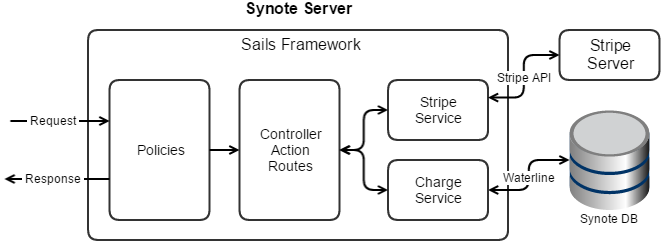
\includegraphics[width=\textwidth]{synote-stripe-overview.png}
  	\caption{Overview Of Synote-Stripe Architecture}
 	\label{fig:synote-stripe}
\end{figure}

\section{Server Side Testing}
\label{sec:server-side-testing}

Testing is crucial in order to provide a robust and reliable feature. The existing testing strategy in Synote's server code uses Mocha \cite{mocha} test running framework paired with Chai \cite{chai} assertion library. Unit, Integration and server side end-to-end (E2E) tests have been written for the payment feature. Through use of Istanbul \cite{istanbul} code coverage tool, we can show high coverage in policies, services and the controller as shown in \textbf{Figure \ref{fig:coverage}}. To thoroughly test our implementation we have written tests for presence, edge-cases and branch coverage. A collection of tests from \texttt{StripeService.test.js} are shown in \textbf{Listing \ref{lst:stripe-test-cases}}.\\

\begin{figure}[!hbt]
  	\centering
 	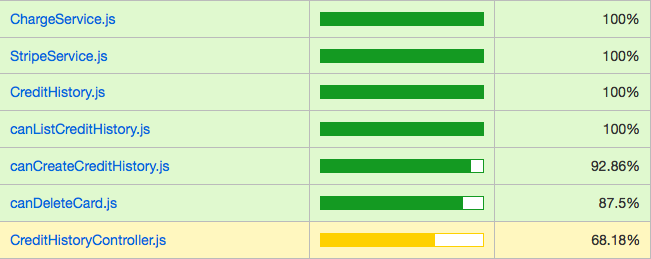
\includegraphics[width=0.9\textwidth]{coverage-all.png}
  	\caption{Istanbul Coverage Report Section}
 	\label{fig:coverage}
\end{figure}

As we were using some of the required technologies for the first time, we had to follow a cycle of prototype-test-refactor meaning we were unable to perform test driven development. Writing tests as part of the development process helped us to spot errors early and know when to change approaches or simply refactor. Where appropriate, tests were actually written by another team member in parallel with development and our client reviewed our code each week ensuring all code is tested and reviewed.\\

\begin{listing}[H]
\begin{minted}[xleftmargin=\parindent, linenos, breaklines, breakanywhere, bgcolor=lightgray, fontsize=\small]{js}
it('Should throw error "Invalid positive integer" when a negative cost is used', function (done) {...});

it('Should throw error "Amount must be at least 30 pence" when a "too low" cost is used', function (done) {...});

it('Should throw error "Invalid integer: text" when "text" cost is used', function (done) {...});

it('Should throw error "No such customer: badValue" when "badValue" customer is provided', function (done) {...});

it('Should throw error "chargeCard: Missing properties in provided JSON" when no customer is provided', function (done) {...});

\end{minted}
\captionof{listing}{Section Of \texttt{StripeService.test.js}}
\label{lst:stripe-test-cases}
\end{listing}

All test cases attempt to follow the SILO and DRY (Don't Repeat Yourself) principles to ensure each case is independent. While SILO has been completely achieved, DRY has not as the existing testing strategy for policies and controllers has forced code repetition. At present \texttt{policy} and \texttt{controller} files are being tested through endpoint calls which is not considered best practice and results in some code branches not being testable. The desired methodology for testing \texttt{policy} files is to do so in isolation using mocking for \texttt{req} objects and spies for function calls. We have included an example of this in \texttt{canListCreditHistory.text.js} in Synote's repository. Best practice for testing \texttt{controllers} and \texttt{services} is to use dependency injection to remove interaction with a real database and \texttt{http} context. This is far beyond the scope of our project but is recommended as future improvement for Synote.

\section{Client Side Implementation}
\label{sec:client-side-implementation}

\subsection{Wireframes}
\label{subsec:wireframes}

First step in design was to mock up some wireframes and get them approved by our Client. Consider the final wireframe iterations below:\\

\begin{figure}[!hbt]
  	\centering
 	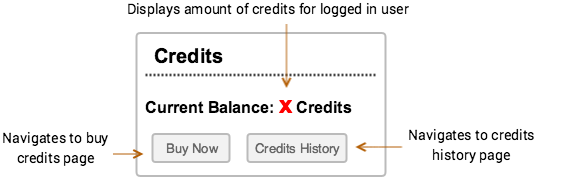
\includegraphics[width=0.7\textwidth]{profile-page-payment-feature.png}
  	\caption{Profile Page Payment and Credits Section Wireframe}
 	\label{fig:profile-wireframe}
\end{figure}

\begin{figure}[!hbt]
  	\centering
 	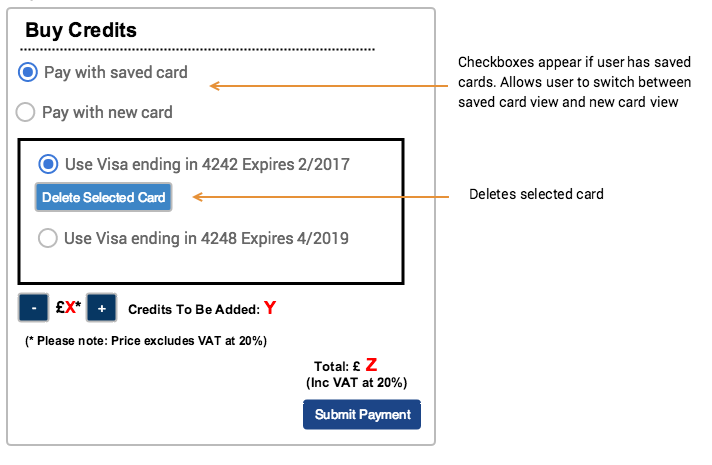
\includegraphics[width=0.8\textwidth]{saved-card-wireframe.png}
  	\caption{Saved Card Payment Form Wireframe}
 	\label{fig:saved-card-wireframe}
\end{figure}

\begin{figure}[!hbt]
  	\centering
 	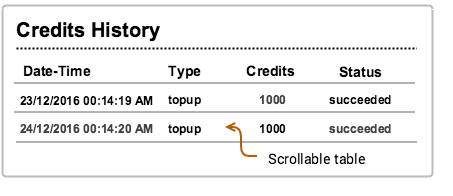
\includegraphics[width=0.6\textwidth]{credits-history-wireframe.png}
  	\caption{Credits History Wireframe}
 	\label{fig:credits-history-wireframe}
\end{figure}

\begin{figure}[!hbt]
  	\centering
 	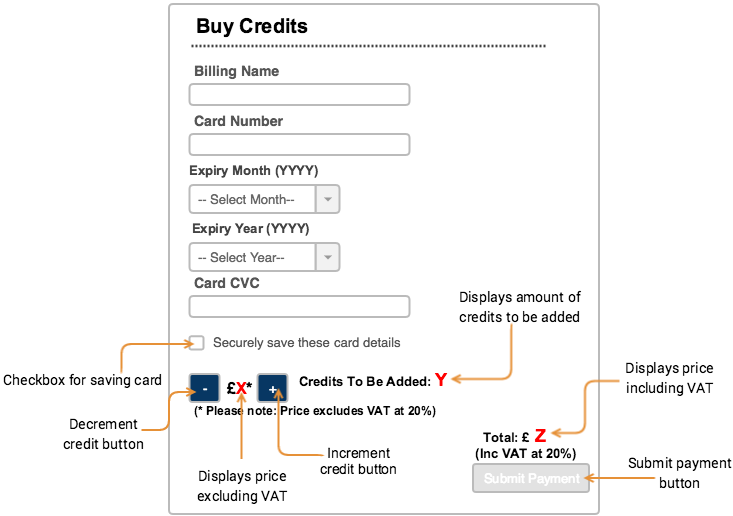
\includegraphics[width=0.8\textwidth]{payment-form-wireframe.png}
  	\caption{Payment Form Wireframe}
 	\label{fig:payment-form-wireframe}
\end{figure}

\subsection{Payment System Infrastructure (Frontend)}
\label{subsec:payment-system-infrastructure}

\begin{figure}[!hbt]
  	\centering
 	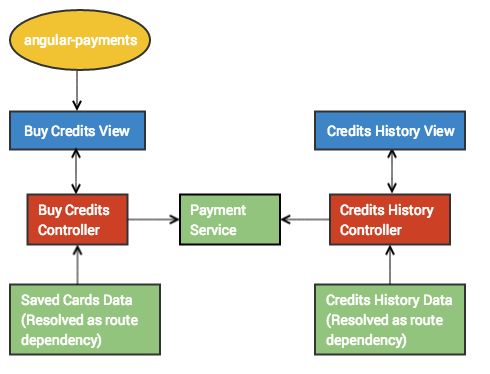
\includegraphics[width=0.6\textwidth]{frontend-infrastructure.png}
  	\caption{Frontend Infrastructure}
 	\label{fig:frontend-infrastructure-diagram}
\end{figure}

Client side should handle these properties of the payment feature:

\begin{itemize}
\item Displaying credits history of logged in user
\item Redemption of credits via new card
\item Redemption of credits via saved card
\item Deletion of saved cards
\item Validation messages
\end{itemize}

“Credits History” and “Buy Credits” are very different components of the payment feature, so we created 2 separate controllers i.e. \texttt{buyCreditController} and \texttt{creditsHistoryController} to handle their logic independently.

\subsubsection{Buy Credits Feature}
\label{subsubsec:buy-credits-feature}

As mentioned in \textbf{Figure \ref{fig:simple-sequence}}, it is the client application's responsibility to tokenise payment data and handle the response from Stripe. The \texttt{buyCreditController} handles all the payment related business logic with the help of \texttt{paymentService} service class (see \textbf{Figure \ref{fig:frontend-infrastructure-diagram}}). This class provides the \texttt{buyCreditController} with:

\begin{itemize}
\item Stripe tokenisation and response handler methods
\item Payment form input validation methods
\item Charge card method (server request)
\item Delete card method (server request)
\end{itemize}

Initially, all of this logic was handled by the \texttt{buyCreditController} itself and this lead to lot of code repetition. Doing simple things like changing the POST request URL for charging a card proved to be a hassle since we had to make these changes at multiple locations. We refactored all the reusable functions into \texttt{paymentService} making simplifying service updates. \\

To use \texttt{Stripe.js} on client side, we first had to include its library as a script in the \texttt{index.html} page. Consider \textbf{Listing \ref{lst:index-head-html}}:\\

\begin{listing}[H]
\begin{minted}[xleftmargin=\parindent, linenos, breaklines, breakanywhere, bgcolor=lightgray, fontsize=\small]{html}
<head>
 <meta charset="utf-8">
 <title>Synote</title>
 <!-- code omitted -->
 <script type="text/javascript" src="https://js.stripe.com/v2/"></script>
 <!-- code omitted -->
</head>
\end{minted}
\captionof{listing}{Section of \texttt{index.html} file}
\label{lst:index-head-html}
\end{listing}

We also had to include our actual publishable API key as a script which will be used to identify Synote to Stripe when sending requests. Consider \textbf{Listing \ref{lst:buycredit-html-stripe-key}}:\\

\begin{listing}[H]
\begin{minted}[xleftmargin=\parindent, linenos, breaklines, breakanywhere, bgcolor=lightgray, fontsize=\small]{html}
//code omitted
<script type="text/javascript">
  Stripe.setPublishableKey('<pk_test_key_here>');
</script>
<!-- code omitted -->
\end{minted}
\captionof{listing}{Section of \texttt{buycredit.html} file}
\label{lst:buycredit-html-stripe-key}
\end{listing}

Payment can be of 2 forms - via a saved card or via a new card.\\

We had to ensure side secure transmission of card details from client i.e. they should not be intercepted and manipulated by an outsider. To achieve this level of security, we tokenise the critical payment fields via Stipe’s API and post this to Synote’s server along with other details such as amount of credits and price to pay. This way, we can assure that original customer details will not be sent to the server.\\

\texttt{paymentService} is responsible for converting the user input payment details into a single use representative token.  Consider \textbf{Listing \ref{lst:create-token-payment-service-method}}:\\

\begin{listing}[H]
\begin{minted}[xleftmargin=\parindent, linenos, breaklines, breakanywhere, bgcolor=lightgray, fontsize=\small]{js}
//code omitted
createStripeToken: function (tokenHelperObject) {

  //the object which will create and manage the promise
  var deferred = $q.defer();

  Stripe.card.createToken(tokenHelperObject,
    function (status, response) {

      if (response.error) {
        //if createToken method fails, reject the promise
        deferred.reject(response.error);
      } else {
        //if the createToken method succeeds, resolve the promise
        deferred.resolve(response);
    }});

    return deferred.promise;//return the promise
},
//code omitted
\end{minted}
\captionof{listing}{Section of \texttt{paymentservice.js} file}
\label{lst:create-token-payment-service-method}
\end{listing}

The method provided by Stripe’s API is \texttt{Stripe.Card.createToken} (line 4). This is in callback style and Synote’s conventions (see \textbf{Section \ref{subsec:conventions}}) favours promises over callbacks. Our \texttt{createStripeToken} method uses Angular’s \texttt{\$q} constructor service to to turn callbacks into promises \cite{jdotjdot} \& \cite{angularjsq}. The token helper object consists of input payment details i.e. billing name, number, cvc, expiry month and year.\\

If the response from Stripe was successful, \texttt{buyCreditController} will then move onto processing the payment via \texttt{paymentService}. Consider \textbf{Listing \ref{lst:charge-card-service-method}}:\\

\begin{listing}[H]
\begin{minted}[xleftmargin=\parindent, linenos, breaklines, breakanywhere, bgcolor=lightgray, fontsize=\small]{js}
//code omitted
chargeCard: function (parameters) {
  return $http({
    url: ENV.apiEndpoint + '/CreditHistory/topup',
    method: 'POST',
    data: parameters
  });
},
//code omitted
\end{minted}
\captionof{listing}{Section of \texttt{paymentservice.js} file}
\label{lst:charge-card-service-method}
\end{listing}

Here we simply make a post request to Synote’s server at \texttt{topup} endpoint along with the single use representative token, credits, charge amount, save boolean as parameters. 'Save boolean flag' is set true if user checks the save card option. It tells the server to save the card currently used for payment.\\

The logic behind is similar to using a new card apart from the fact that we no longer need to tokenise the payment details. When user is routed to the \texttt{buycredit} URI, we send a HTTP GET request to Synote’s server to retrieve saved cards for logged-in users (see \textbf{Figure \ref{fig:frontend-infrastructure-diagram}}). Consider \textbf{Listing \ref{lst:get-cards-req}}:\\

\begin{listing}[H]
\begin{minted}[xleftmargin=\parindent, linenos, breaklines, breakanywhere, bgcolor=lightgray, fontsize=\small]{js}
//code omitted
cards: ['$http', 'authenticationService',
  function ($http, authenticationService) {
    var usrId = authenticationService.getUserInfo().user_id;
    return $http({
      url: ENV.apiEndpoint + '/creditHistory/cards',
      method: "GET"
    });
}]
//code omitted
\end{minted}
\captionof{listing}{Section of \texttt{app.js} file}
\label{lst:get-cards-req}
\end{listing}

When charging against saved card, we invoke the same method from \texttt{paymentService} used for charging against a new card but with different parameters. Consider \textbf{Listing \ref{lst:params-charge-card}}:\\

\begin{listing}[H]
\begin{minted}[xleftmargin=\parindent, linenos, breaklines, breakanywhere, bgcolor=lightgray, fontsize=\small]{js}
//code omitted
var parameters = {
  useSavedCard: $scope.useSavedCard,
  cardId: $scope.cardChoosen.card ? $scope.cardChoosen.card.id : null,
  tokenResponse: $scope.useSavedCard ? null : token,
  save: $scope.saveCard,
  amount: $scope.currentPriceTotalIncludingVAT,
  credits: $scope.currentCreditsTotal
};
//code omitted
\end{minted}
\captionof{listing}{Section of \texttt{buycredit.js} file}
\label{lst:params-charge-card}
\end{listing}

Instead of passing in the Stripe token, we now pass the \texttt{cardId} of selected card.

\subsubsection{Credits History Feature}
\label{subsubsec:credits-history-feature}

When users are routed to the \texttt{creditsHistory} URI, we send a HTTP GET request to Synote’s server to retrieve credit history for logged in user. Consider \textbf{Listing \ref{lst:credits-history-req}}:\\

\begin{listing}[H]
\begin{minted}[xleftmargin=\parindent, linenos, breaklines, breakanywhere, bgcolor=lightgray, fontsize=\small]{js}
//code omitted
creditHistory: ['$http', 'authenticationService',
  function ($http, authenticationService) {
    var usrId = authenticationService.getUserInfo().user_id;
    return $http({
      url: ENV.apiEndpoint + '/creditHistory/history',
      method: "GET"
    });
}]
//code omitted
\end{minted}
\captionof{listing}{Section of \texttt{app.js file}}
\label{lst:credits-history-req}
\end{listing}

The loaded credit history data is then displayed as a reverse chronological table.

\subsection{Clientside Payment Details Validation}
\label{subsec:clientside-payment-details-validation}

Client side validation is handled via methods provided by Stipe’s API and an Angular payment validation module  (see \textbf{Figure \ref{fig:frontend-infrastructure-diagram}}) called \texttt{angular-payments} \cite{angularpayments}. Stripe’s validation methods are called via \texttt{buycredit.html} page $>$ \texttt{buycredit} controller $>$ \texttt{paymentservice} service. Consider validation for card number field as an example:

\begin{listing}[H]
\begin{minted}[xleftmargin=\parindent, linenos, breaklines, breakanywhere, bgcolor=lightgray, fontsize=\small]{html}
<!-- code omitted -->
<input class="form-control" name="number" payments-format="card" ng-model="cardNumber" ng-paste="$event.preventDefault()" ng-change="checkCardNumber()" required>
<!-- code omitted -->
\end{minted}
\captionof{listing}{Section of \texttt{buycredit.html file}}
\label{lst:buycredit-html-cardnumber-input}
\end{listing}

In \textbf{Listing \ref{lst:buycredit-html-cardnumber-input}}, we  use Angular’s \texttt{ng-change} directive to execute \texttt{checkCardNumber} method whenever it detects an input change e.g. keypress. \texttt{payments-format=”card”} is provided by \texttt{angular-payments} and ensures input to be 16 digits maximum.\\

\begin{listing}[H]
\begin{minted}[xleftmargin=\parindent, linenos, breaklines, breakanywhere, bgcolor=lightgray, fontsize=\small]{js}
//code omitted
$scope.checkCardNumber = function () {
  if ($scope.cardNumber) {
    $scope.theForm.number.setValidity("minLength",
      paymentService.isCardNumberTypeValid($scope.cardNumber));
  }
};
//code omitted
\end{minted}
\captionof{listing}{Section of \texttt{buycredit.js} file}
\label{lst:buycredit-controller-checkcardnumber-method}
\end{listing}

In \textbf{Listing \ref{lst:buycredit-controller-checkcardnumber-method}}, we check validity of the payment form based on the input card number via \texttt{paymentService}.\\

\begin{listing}[H]
\begin{minted}[xleftmargin=\parindent, linenos, breaklines, breakanywhere, bgcolor=lightgray, fontsize=\small]{js}
//code omitted
isCardNumberTypeValid: function (cardNumber) {
  var cardType = Stripe.card.cardType(cardNumber);
  var validCardNumBool = Stripe.card.validateCardNumber(cardNumber);
  return validCardNumBool && !(cardType === 'undefined');
},
//code omitted
\end{minted}
\captionof{listing}{Section of \texttt{paymentservice.js} file}
\label{lst:payment-service-checkcardnumber-method}
\end{listing}

In \textbf{Listing \ref{lst:payment-service-checkcardnumber-method}}, we use Stripe provided methods to validate provided card number.\\

\begin{figure}[!hbt]
  	\centering
 	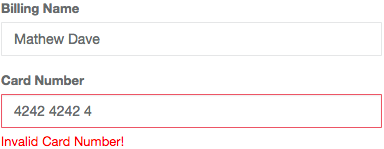
\includegraphics[width=0.6\textwidth]{live-validation-screenshot.png}
  	\caption{Live Validation In Action}
 	\label{fig:live-validation-screenshot}
\end{figure}

\subsection{Alert Messages}
\label{subsec:alert-messages}

Synote uses \texttt{Toastr} alert messages throughout its implementation. An issue arose whilst writing automated E2E tests where the \texttt{Toastr} alerts would prevent WebDriver from accessing the logout button. Consider \textbf{Figure \ref{fig:toastr-alert-problem-screenshot}}:\\

\begin{figure}[!hbt]
  	\centering
 	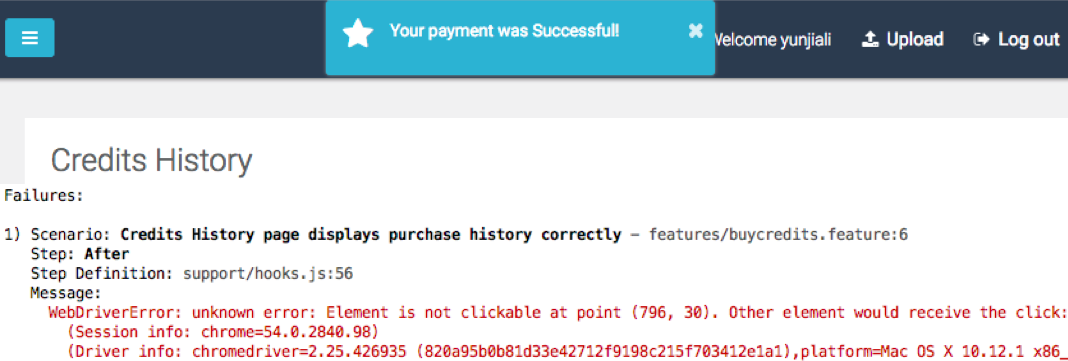
\includegraphics[width=\textwidth]{toastr-alert-problem-screenshot.png}
  	\caption{Example of Error Caused by \texttt{Toastr} Alerts}
 	\label{fig:toastr-alert-problem-screenshot}
\end{figure}

To overcome this issue, we switched to Bootstrap alerts which are added on the fly and set to disappear after 5 seconds. Consider \textbf{Listing \ref{lst:buycredit-html-alert-code}}:\\

\begin{listing}[H]
\begin{minted}[xleftmargin=\parindent, linenos, breaklines, breakanywhere, bgcolor=lightgray, fontsize=\small]{html}
<!-- code omitted -->
<uib-alert dismiss-on-timeout="5000" ng-repeat="alert in alerts|limitTo:4" type="{{alert.type}}" close="closeAlert($index)">
  <strong>{{ alert.title }}</strong> {{ alert.msg }}
</uib-alert>
<!-- code omitted -->
\end{minted}
\captionof{listing}{Section of \texttt{buycredit.html} file}
\label{lst:buycredit-html-alert-code}
\end{listing}

\begin{figure}[!hbt]
  	\centering
 	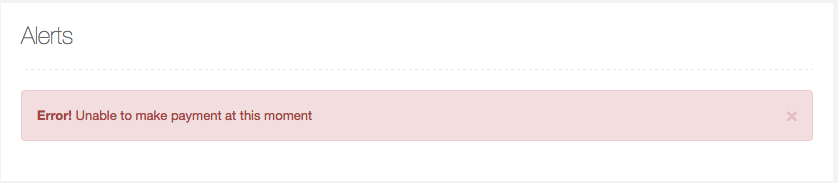
\includegraphics[width=0.8\textwidth]{alert-fail.png}
  	\caption{Alert Shown When Payment Couldn't Be Processed}
 	\label{fig:alert-success}
\end{figure}

\begin{figure}[!hbt]
  	\centering
 	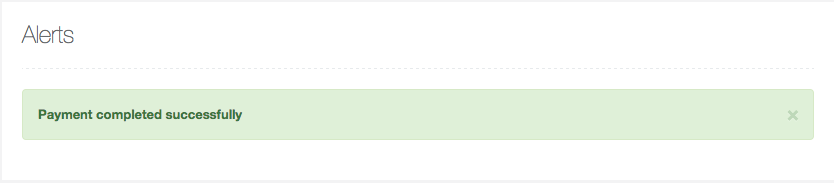
\includegraphics[width=0.8\textwidth]{alert-success.png}
  	\caption{Alert Shown When payment Was Successful}
 	\label{fig:alert-fail}
\end{figure}

\subsection{Responsive Design}
\label{subsec:responsive-design}

To fit in with the responsive style of Synote, Bootstrap framework was used and the responsiveness of view files we added were tested using Firefox’s responsive design mode \cite{firefoxresponsive} which let us emulate screen sizes of different devices. Consider the screenshots of tests in action:\\

\begin{figure}[!htb]
    \centering
    \begin{minipage}{.45\textwidth}
        \centering
        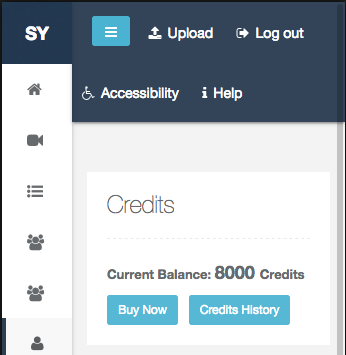
\includegraphics[width=\textwidth]{responsive-profile-page.png}
          \caption{Profile Page Responsive View}
        \label{fig:responsive-profile}
        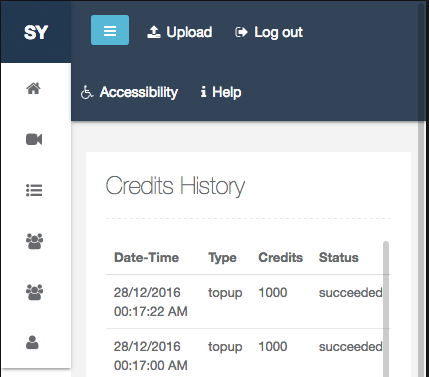
\includegraphics[width=\textwidth]{responsive-credits-history.png}
          \caption{Credits History Responsive View}
        \label{fig:responsive-credits-history}
    \end{minipage}%
    \hspace{0.1cm}
    \begin{minipage}{0.5\textwidth}
        \centering
        \centering
      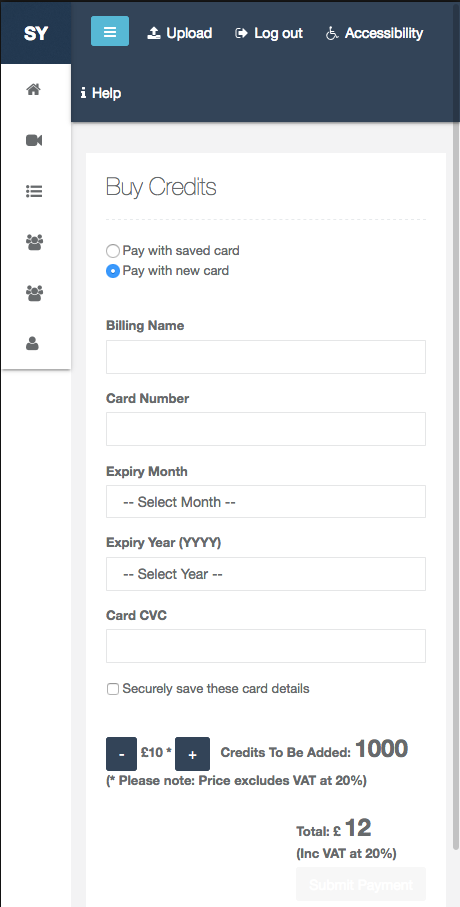
\includegraphics[width=\textwidth]{responsive-payment-form.png}
        \caption{Payment Form Responsive View}
      \label{fig:responsive-payment-form}
    \end{minipage}
\end{figure}

\chapter{E2E Test Framework}
\label{chap:e2e-test-framework}

\section{Automated E2E Testing}
\label{sec:automated-e2e-testing}

\subsection{Manual vs Automatic E2E Testing}
\label{sec:manual-vs-automatic-e2e-testing}

\subsection{Technologies Used}
\label{sec:technologies-used}

\section{Test Framework Components}
\label{sec:test-framework-components}

\subsection{Feature Definition as Requirements}
\label{subsec:feautre-definition-as-requirements}

Feature files can be seen as an entry point to cucumber test cases \cite{featurefile1}. Each of the feature file should be written to test a single feature of the application or a particular area of feature \cite{featurefile2}. Since we were writing E2E tests for the payment feature, we created \texttt{buycredits.feature} file for testing this aspect. Consider \textbf{Listing \ref{lst:buycredits-feature-file}}:\\

\begin{listing}[H]
\begin{minted}[xleftmargin=\parindent, linenos, breaklines, breakanywhere, bgcolor=lightgray, fontsize=\small]{cucumber}
@dev @experiment
Feature: Buying Credit feature
  As a user of Synote
  I should be able to successfully buy credits when logged in

  Scenario: Access buy credits page when logged in
    Given I click the "Profile" button on "SideMenu" page
    Given I click the "BuyCredit" button on "Profile" page
    Then I should be on "BuyCredits" page

  Scenario: Buy credit with empty card number
    Given I click the "Profile" button on "SideMenu" page
    Given I click the "BuyCredit" button on "Profile" page
    Given I Correctly type in my details but "" for "number"
    Then Submit button should be disabled
# code omitted
\end{minted}
\captionof{listing}{Section of \texttt{buycredits.feature} file}
\label{lst:buycredits-feature-file}
\end{listing}

The section in \textbf{Listing \ref{lst:buycredits-feature-file}} is written in a language called \texttt{Gherkin}. \texttt{Gherkin} makes use of Business Readable Domain Specific Language (BRDSL) which allows us to write the test cases at a business level without getting into implementation details.

Our client required us to document the requirements/specification for the new payment feature. Most of Synote's team are developers and since the feature file used \texttt{Gherkin}, it was readable on a business level and could act as automation test script \cite{featurefile1}. Hence, we recommended using the feature files themselves as the requirements documentation.\\

Each of the feature file should be defined with \texttt{Feature} keyword which consists of a name  (see \textbf{Listing \ref{lst:buycredits-feature-file}} line  2) and brief description  (see \textbf{Listing \ref{lst:buycredits-feature-file}} line  3-4). Each of the test cases are defined with \texttt{Scenario} keyword followed by a brief description of that test (see \textbf{Listing \ref{lst:buycredits-feature-file}} line  6 and 11). Each scenario should \cite{featurefile3}:
\begin{itemize}
\item Describe event taking place
\item Describe expected result
\end{itemize}

We use \texttt{Steps} to achieved this. Consider the \texttt{Access buy credits page when logged in} scenario in \textbf{Listing \ref{lst:buycredits-feature-file}}. We use keywords such as \texttt{Given} (line 7 and 8), \texttt{Then} (line 9) for writing readable test cases. Consider \textbf{Table \ref{tab:steps-keywords}} which define \texttt{Step} keywords \cite{featurefile1}

\begin{center}
%Column widths dependent on page width/margins
\begin{tabular}{ |p{2cm}|p{7cm}| }

 \hline
 	Keyword &
 	Description\\
 \hline
 	Given & Describes test pre-condition\\
 \hline
 	And & Defines additional test conditions\\
 \hline
 	Then & Defines expectations of test \\
 \hline

\end{tabular}
\captionof{table}{\texttt{Step keywords}}
\label{tab:steps-keywords}
\end{center}

\subsection{Reusable Steps Definition}
\label{subsec:reusable-steps-definition}

Cucumber is not able to execute the scenarios as they are. Instead, we have to write \texttt{step} definitions. Step definitions use regular expression to map the \texttt{Gherkin steps} to actions which will drive system interactions \cite{stepfile1}. Each of the \texttt{steps} written for scenarios in the \texttt{feature} file should have a \texttt{step} definition declared in its corresponding \texttt{step} file.\\ A \texttt{step} file should only contain definitions for \texttt{steps} used in corresponding \texttt{feature} file. Consider \textbf{Listing \ref{lst:buycredits-step-file}}:\\

\begin{listing}[H]
\begin{minted}[xleftmargin=\parindent, linenos, breaklines, breakanywhere, bgcolor=lightgray, fontsize=\small]{js}
@dev @experiment
//code omitted
this.Given(/^I click the "([^"]*)" button on "([^"]*)" page$/,
  function (buttonName, pageName) {
    return this.Support.clickButton(buttonName, pageName);
});

this.Given(/^I should be on "([^"]*)" page$/, function (pageName) {
  return this.Support.waitUntil
      (this.Support.urlChanged(this.Support.getPageUrl(pageName))
    , 2000)();
});
//code omitted
\end{minted}
\captionof{listing}{Section of \texttt{buycredits.steps.js} file}
\label{lst:buycredits-step-file}
\end{listing}

In our case, all the \texttt{steps} written in \texttt{buycredits.feature} file are defined in the \texttt{buycredits.steps.js} file. Each step should have a unique definition else an \texttt{ambiguous match} exception will be thrown. \textbf{Listing \ref{lst:buycredits-step-file}} contains the step definitions for \texttt{Access buy credits page when logged in} scenario in \textbf{Listing \ref{lst:buycredits-feature-file}}. Inside the step definitions, we write javascript code to handle the interaction logic e.g. 1st definition in \textbf{Listing \ref{lst:buycredits-step-file}} (line 3) handles clicking of button provided  \texttt{buttonName and pageName} parameters and 2nd definition (line 7) handles checking we are on a page with certain URL provided  \texttt{pageName} parameter. Nearly all of out step definitions take parameters instead of hard-coding them. This way, we can satisfy the \texttt{DRY} principle by reusing generic step definitions, making both  \texttt{feature} and  \texttt{step} files easily maintainable and readable in the long run.

\subsection{Reusable Support Functions}
\label{subsec:reusable-support-functions}

In order to have generic \texttt{step} definitions (e.g. see \textbf{Listing \ref{lst:buycredits-step-file}} line 3 and 7), we needed to write common generic methods which will drive interactions with the system. We place such functions in the \texttt{support.js} file. As a rule of thumb, we identified generic methods to go in the \texttt{support.js} file by checking if were were repeating any code/logic in the \texttt{bycredits.steps.js} file. Currently, our frame work uses the \texttt{support.js} file for:

\begin{itemize}
\item Clicking
\item Filling inputs
\item Navigating
\item Data retrieval
\end{itemize}

\begin{listing}[H]
\begin{minted}[xleftmargin=\parindent, linenos, breaklines, breakanywhere, bgcolor=lightgray, fontsize=\small]{js}
@dev @experiment
//code omitted
function loadPageOnSupport(pageName) {
  if (!support[pageName]) {
    support[pageName] = require
      ('../pages/' + pageName.toLowerCase() + '.page.js');
  }
}
//code omitted
fillInputOnPage: function (pageName, textBox, text) {
  loadPageOnSupport(pageName);
  if (this[pageName] && this[pageName][textBox + 'Input']) {
    var _textBox = this[pageName][textBox + 'Input'];
    return _textBox.sendKeys(text);
  }
}
//code omitted
\end{minted}
\captionof{listing}{Section of \texttt{support.js} file}
\label{lst:support-file-methods}
\end{listing}

Consider \textbf{Listing \ref{lst:support-file-methods}}. The \texttt{fillInputOnPage} is a common generic method i.e. it can be used to fill any input field on any page, hence its placement in the \texttt{support.js} file. The \texttt{loadPageOnSupport} method helps \texttt{support.js} file to be generic in applying its methods in different contexts by dynamically requiring desired pages objects. Main advantage of \texttt{support.js} is that testers will never have to rewrite any code they have already written, satisfying the \texttt{DRY} principle.

\subsection{Pre and Post Hooks}
\label{subsec:pre-and-post-hooks}

\subsection{Page Objects}
\label{subsec:page-objects}
There are few key interactions which are very common throughout the application e.g. clicking buttons, filling in inputs, navigating to pages etc. It seemed tedious and time consuming to actually write separate methods for these interactions on different pages. We came to the conclusion that the interactions themselves should be generic enough so they can be applied to any page. The pages of application differed in the elements and components they had. Hence, we have definitions of \texttt{Page Object Models} which is composed of elements a page has.

\begin{minipage}{.48\textwidth}
\begin{listing}[H]
\begin{minted}[xleftmargin=\parindent, linenos, breaklines, breakanywhere, bgcolor=lightgray, fontsize=\small]{js}
{ // buyCredits.page.js snippet
Title : "BuyCredits",
Url : browser.deployment.hostUrl + 'buycredit',

billing_nameInput : element
  (by.model('billingName')),

numberInput : element
  (by.model('cardNumber')),

cvcInput : element
  (by.model('cardCVC')),

exp_monthInput : element
  (by.model('expMonth')),

exp_yearInput : element
  (by.model('expYear')),

PaySavedRadioButton : element
  (by.id('pay-saved-radio')),
//code omitted
}
\end{minted}
\captionof{listing}{Section of \texttt{buycredits.page.js} file}
\label{lst:buycredits-page-code}
\end{listing}
\vspace{0.1cm}
\end{minipage}%
\begin{minipage}{.49\textwidth}
  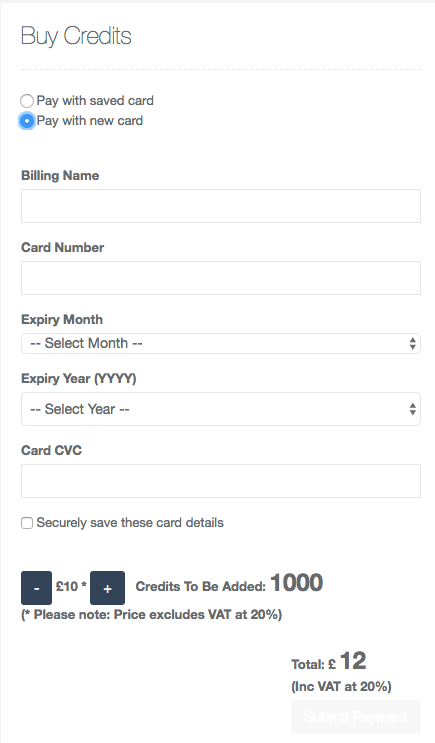
\includegraphics[width=\textwidth]{screenshot-payment-form.png}
  \captionof{figure}{Payment Form}
 	\label{fig:paymentform-screenshot}
\end{minipage}

Here you have the \texttt{buycredits.html} page (\textbf{Figure \ref{fig:paymentform-screenshot}}) and it has a corresponding \texttt{buycreditspage.js} \textit{page object file} (\textbf{Listing \ref{lst:buycredits-page-code}}) which is basically a one to one mapping from the html page components. Page object files also house methods to interact with elements (defined in the same \textit{page object model}) which are only applicable to the particular page in question e.g. \texttt{buycreditspage.js} has a method called \texttt{fillDefaultCardDetails} which fills in the payment form fields and is only applicable to \texttt{buycredits.html} page. The main advantages of implementing page objects were reduced code duplication and easy maintainability i.e.  if any of the UI element of the application was changed, we only have to modify them in the page object file instead of fixing them in each \texttt{step} which used that UI element \cite{semaphore}. Another advantage is that it structures the framework, improving readability.

\subsection{Deployment Definition}
\label{subsec:deployment-definition}

\subsection{Reporting}
\label{subsec:reporting}

\subsection{Assessment}
\label{subsec:assessment}

\chapter{Continuous Integration}
\label{chap:continuous-integration}

The final phase of our project was to implement a continuous integration (CI) process for Synote. Only by deploying a new version of Synote and testing it can we be sure that a feature implementation is stable and functioning. However, a Synote experiment deployment has quite a few steps (\textbf{Figure \ref{fig:synote-ci-proc}}), which can take 15-30 minutes. In fact, it is completely infeasible to regularly repeat all the steps without hampering a developer's work. Since making a deployment takes  considerable time and is incredibly useful in continuous automated testing on remote deployments, we extended our project scope to implement Synote's first continuous integration process.

\section{Synote CI}
\label{sec:synote-ci}

A complete Synote CI process will deploy and test on the experiment deployment, followed by staging and finally production. Each stage will follow similar steps as Step 2 or the Experiment Deployment.

\begin{figure}[!hbt]
  	\centering
 	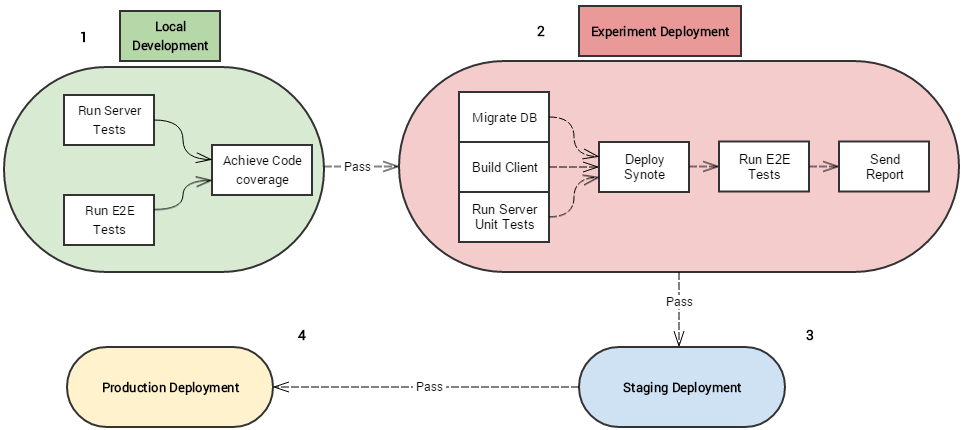
\includegraphics[width=\textwidth]{synote-ci.png}
  	\caption{Synote Continuous Integration Procedure}
 	\label{fig:synote-ci-proc}
\end{figure}

We focused on CI for the experiment deployment since we had access to it. In this chapter, we will elucidate the key steps necessary to configure a complete CI environment using Jenkins.\\

The key issues in this phase were -

\begin{itemize}

  \item Installing and configure Jenkins with SSL, restricted user access etc. (\textbf{Section \ref{subsec:setting-up-jenkins}})

  \item Synote is deployed as user \texttt{ubuntu}, however, Jenkins runs the build scripts as user \texttt{jenkins}. So, permissions for the deployment folders need to be rectified (\textbf{Listing \ref{lst:deployment-folder-permissions}}).

  \item \texttt{jenkins} needs to have access to the PM2 (a process manager) processes started by \texttt{ubuntu} (\textbf{Listing \ref{lst:jenkins-pm2-configuration}}).

  \item Running the E2E tests on a browser using a virtual display (\textbf{Section \ref{subsec:e2e-testing-on-remote}}).

\end{itemize}

\subsection{Setting up Jenkins}
\label{subsec:setting-up-jenkins}

We began by installing Jenkins on the experiment server (\textbf{Listing \ref{lst:install-jenkins}}). After monitoring the processes, we asked the client to upgrade the server to have 4GB RAM.

\begin{listing}[H]
\begin{minted}[xleftmargin=\parindent, linenos, breaklines, breakanywhere, bgcolor=lightgray, fontsize=\small]{bash}

# install Jenkins on Ubuntu (Synote Experiment Deployment)
wget -q -O - https://pkg.jenkins.io/debian/jenkins-ci.org.key | sudo apt-key add -
sudo sh -c 'echo deb http://pkg.jenkins.io/debian-stable binary/ > /etc/apt/sources.list.d/jenkins.list'
sudo apt-get update
sudo apt-get install jenkins

\end{minted}
\captionof{listing}{Install Jenkins}
\label{lst:install-jenkins}
\end{listing}

Then we added one admin account with complete Jenkins control, and one developer account with reduced control (e.g. cannot delete projects). Finally, we needed to run Jenkins behind a reverse proxy server (nginx) so that SSL encryption works properly and the domain reaches it (\textbf{Listing \ref{lst:make-jenkins-available}}). The Synote experiment CI project can be seen in \textbf{Figure \ref{fig:synote-jenkins-server}}

\begin{listing}[H]
\begin{minted}[xleftmargin=\parindent, linenos, breaklines, breakanywhere, bgcolor=lightgray, fontsize=\small]{bash}

# nginx reverse proxy configuration for Jenkins

echo "upstream jenkins {
  server 127.0.0.1:8080 fail_timeout=0;
}

server {
  listen 80;
  server_name jenkins-cicd.synote.com; # dns for Synote CI
  return 301 https://$host$request_uri;
}

# ssl redirection

server {
  listen 443 ssl;
  server_name <synote_jenkins_ci_domain_name>;

  ssl_certificate <synote_ssl_certificate_location>;
  ssl_certificate_key <synote_ssl_private_key_location>;

  location / {
    proxy_set_header        Host $host:$server_port;
    proxy_set_header        X-Real-IP $remote_addr;
    proxy_set_header        X-Forwarded-For $proxy_add_x_forwarded_for;
    proxy_set_header        X-Forwarded-Proto $scheme;
    proxy_redirect http:// https://;
    proxy_pass              http://jenkins;
  }
}" > /etc/nginx/sites-available/jenkins

sudo service nginx restart

\end{minted}
\captionof{listing}{Make Jenkins server available on nginx}
\label{lst:make-jenkins-available}
\end{listing}

\begin{figure}[!hbt]
  	\centering
 	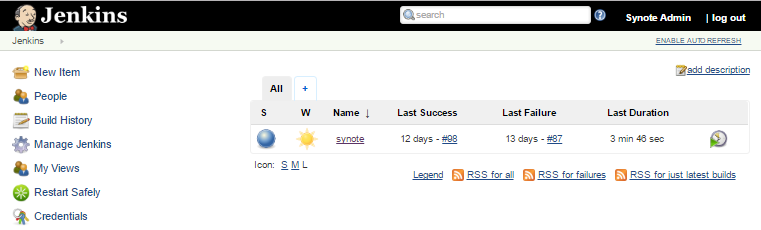
\includegraphics[width=0.78\textwidth]{jenkins.png}
  	\caption{Slack Jenkins Server}
 	\label{fig:synote-jenkins-server}
\end{figure}

\subsection{Triggering Builds}
\label{subsec:triggering-builds}

\begin{figure}[!hbt]
  	\centering
 	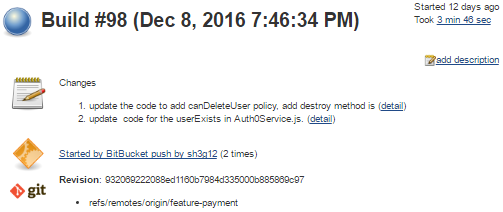
\includegraphics[width=0.78\textwidth]{jenkins-build-trigger.png}
  	\caption{Jenkins Build Trigger}
 	\label{fig:jenkin-build-trigger}
\end{figure}

\section{Pre-build Preparation}
\label{sec:pre-build-preparation}

We first needed to give the ownership of \texttt{npm} modules to \texttt{ubuntu} (\textbf{Listing \ref{lst:npm-permission}}), so that we could install \texttt{bower}, which is needed to resolve the client app dependencies.

\begin{listing}[H]
\begin{minted}[xleftmargin=\parindent, linenos, breaklines, breakanywhere, bgcolor=lightgray, fontsize=\small]{bash}

# give permission to install global npm dependecies
sudo chown -R $USER:$GROUP ~/.npm
sudo chown -R $USER:$GROUP ~/.config

\end{minted}
\captionof{listing}{Global npm dependency permission}
\label{lst:npm-permission}
\end{listing}

\textbf{Listing \ref{lst:jenkins-build-script-variables}} is the different source-code locations on the experiment deployment that concerns the CI script. These will be necessary in the later listings.

\begin{listing}[H]
\begin{minted}[xleftmargin=\parindent, linenos, breaklines, breakanywhere, bgcolor=lightgray, fontsize=\small]{bash}

# the repos
SYNOTE_MAIN=/home/ubuntu/synote
SYNOTE_JENKINS=$WORKSPACE
E2E_JENKINS=$WORKSPACE/../gdp8-synote-e2e-testing
E2E_MAIN=/home/ubuntu/gdp8-synote-e2e-testing
REPORTS_WEBSITE_MAIN=$E2E_MAIN/reportsWebsite

\end{minted}
\captionof{listing}{Variables used during the Jenkins build script}
\label{lst:jenkins-build-script-variables}
\end{listing}

Then we give the permissions for the E2E testing and Synote deployment repo to a group that contains both \texttt{ubuntu} and \texttt{jenkins}. Now \texttt{jenkins} can make place new deployments of Synote.

\begin{listing}[H]
\begin{minted}[xleftmargin=\parindent, linenos, breaklines, breakanywhere, bgcolor=lightgray, fontsize=\small]{bash}

# create user group synote
sudo groupadd synote
sudo usermod -a -G synote jenkins
sudo usermod -a -G synote ubuntu

# permissions for e2e testing
sudo chown -R ubuntu: $E2E_MAIN
sudo chgrp -R synote $E2E_MAIN
sudo chmod -R 777 $E2E_MAIN

# permissions for synote
sudo chown -R ubuntu: $SYNOTE_MAIN
sudo chgrp -R synote $SYNOTE_MAIN
sudo chmod -R 777 $SYNOTE_MAIN

\end{minted}
\captionof{listing}{Deployment folder permissions}
\label{lst:deployment-folder-permissions}
\end{listing}

One issue was that \texttt{git} would regularly create some files that are owned by \texttt{ubuntu} and the files built by \texttt{jenkins} could not replace those. So, we remove the \texttt{.git} folders (\textbf{Listing \ref{lst:deleting-git-folders}}), since the more recent versions will be put in there place by \texttt{jenkins} anyway.

\begin{listing}[H]
\begin{minted}[xleftmargin=\parindent, linenos, breaklines, breakanywhere, bgcolor=lightgray, fontsize=\small]{bash}

# delete the .git folders from both repos
# since it creates files for ubuntu account only
rm -rf $SYNOTE_MAIN/.git
rm -rf $E2E_MAIN/.git

\end{minted}
\captionof{listing}{Deleting .git folders}
\label{lst:deleting-git-folders}
\end{listing}

Finally, we need to give \texttt{jenkins} access to the deployment processes created by \texttt{ubuntu} so that it could restart them (\textbf{Listing \ref{lst:jenkins-pm2-configuration}}).

\begin{listing}[H]
\begin{minted}[xleftmargin=\parindent, linenos, breaklines, breakanywhere, bgcolor=lightgray, fontsize=\small]{bash}

# Make locally installed programs available to jenkins
export PATH=${PATH}:/home/ubuntu/.nvm/v4.3.2/bin
export PM2_HOME="/home/ubuntu/.pm2"

# Make pm2 tasks started by 'ubuntu' available to 'jenkins'
sudo chmod 777 /home/ubuntu/.pm2/pub.sock
sudo chmod 777 /home/ubuntu/.pm2/rpc.sock

\end{minted}
\captionof{listing}{PM2 configuration for Jenkins}
\label{lst:jenkins-pm2-configuration}
\end{listing}

\section{Synote Build}
\label{sec:synote-build}

Once a build is triggered, Jenkins pulls the latest Synote repository. Then \texttt{jenkins} builds the server (\textbf{Listing \ref{lst:building-synote-server}}), the client (\textbf{Listing \ref{lst:building-synote-client}}) and moves the static assets to \texttt{backend}. Finally, the complete build folder replaces \texttt{ubuntu}'s Synote deployment folder (\textbf{Listing \ref{lst:replace current deployment source}}).

\begin{listing}[H]
\begin{minted}[xleftmargin=\parindent, linenos, breaklines, breakanywhere, bgcolor=lightgray, fontsize=\small]{bash}

# building the server
cd $SYNOTE_JENKINS/backend
npm install

\end{minted}
\captionof{listing}{Building Synote server}
\label{lst:building-synote-server}
\end{listing}

\begin{listing}[H]
\begin{minted}[xleftmargin=\parindent, linenos, breaklines, breakanywhere, bgcolor=lightgray, fontsize=\small]{bash}

# building the client
cd $SYNOTE_JENKINS/frontend
npm install
bower install
grunt build:experiment

\end{minted}
\captionof{listing}{Building Synote client}
\label{lst:building-synote-client}
\end{listing}

\begin{listing}[H]
\begin{minted}[xleftmargin=\parindent, linenos, breaklines, breakanywhere, bgcolor=lightgray, fontsize=\small]{bash}

# replace the assets in /backend with the new frontend build
cp -RT $SYNOTE_JENKINS/frontend/dist/ $SYNOTE_JENKINS/backend/assets/

# Copy the synote repo from 'jenkins' to synote in 'ubuntu'
cp -RT $SYNOTE_JENKINS $SYNOTE_MAIN

\end{minted}
\captionof{listing}{Replace the current experiment deployment source}
\label{lst:replace current deployment source}
\end{listing}

\subsection{Automated Database Migration}
\label{subsec:automated-database-migration}

\begin{listing}[H]
\begin{minted}[xleftmargin=\parindent, linenos, breaklines, breakanywhere, bgcolor=lightgray, fontsize=\small]{bash}

# Run database migration
# Currently it's hardcoded to the latest migration but in the future,
# this should be decided on runtime depending on the database version
cd $SYNOTE/backend/db/migrate
mysql -u synote '-p<mysqlpass>' synote_server_experiment < procedures.sql # update procedures
mysql -u synote '-p<mysqlpass>' synote_server_experiment < v0.9.0-v0.10.0.sql # do migration

\end{minted}
\captionof{listing}{Automated DB Migration}
\label{lst:automated-db-migration}
\end{listing}

\subsection{Restarting the New Build}
\label{subsec:restarting-the-new-build}

PM2 is a process manager that keeps processes alive even when users log off. Synote experiment deployment is kept alive as a PM2 process, which is restarted by \texttt{jenkins} at this stage (\textbf{Listing \ref{lst:restart-experiment-deployment}}).

\begin{listing}[H]
\begin{minted}[xleftmargin=\parindent, linenos, breaklines, breakanywhere, bgcolor=lightgray, fontsize=\small]{bash}

# always use pm2 app name to restart
pm2 restart synote_experiment

\end{minted}
\captionof{listing}{Restart experiment deployment}
\label{lst:restart-experiment-deployment}
\end{listing}

\section{E2E Testing on Remote}
\label{subsec:e2e-testing-on-remote}

In order to run the E2E tests, we first need the latest E2E tests (which are on a different repository) and prepare it for use (\textbf{Listing \ref{lst:configure-latest-e2e-testing-repo}}) in a similar process to Synote deployment (described in \textbf{Section \ref{sec:synote-build}}).

\begin{listing}[H]
\begin{minted}[xleftmargin=\parindent, linenos, breaklines, breakanywhere, bgcolor=lightgray, fontsize=\small]{bash}

# cloning e2e repo
rm -rf $E2E_JENKINS

cd $SYNOTE_JENKINS/..
git clone git@bitbucket.org:sh3g12/gdp8-synote-e2e-testing.git

# copy over the content to 'ubuntu' e2e testing from 'jenkins'
cp -RT $E2E_JENKINS $E2E_MAIN

# install e2e main dependencies
cd $E2E_MAIN
npm install

\end{minted}
\captionof{listing}{Configure the latest E2E testing repository}
\label{lst:configure-latest-e2e-testing-repo}
\end{listing}

Synote's E2E test HTML reports are made available through a simple website (which is deployed by nginx in a similar process to \textbf{Listing \ref{lst:make-jenkins-available}}). This website is packaged with the E2E tests. So, now we should redeploy the latest reporting website (\textbf{Listing \ref{lst:deploy-latest-reporting-website}}).

\begin{listing}[H]
\begin{minted}[xleftmargin=\parindent, linenos, breaklines, breakanywhere, bgcolor=lightgray, fontsize=\small]{bash}

# install reports website dependencies
cd $REPORTS_WEBSITE_MAIN
npm install

# restart the reporting server
pm2 restart reports_website

\end{minted}
\captionof{listing}{Deploy latest reporting website}
\label{lst:deploy-latest-reporting-website}
\end{listing}

However, browsers that are needed to run the E2E tests need a display. So, a virtual display (Xvfb) is installed, along with the helper libraries and finally the browsers themselves are installed (\textbf{Listing \ref{lst:xvfb-browser-install}}).

\begin{listing}[H]
\begin{minted}[xleftmargin=\parindent, linenos, breaklines, breakanywhere, bgcolor=lightgray, fontsize=\small]{bash}

# install virtual display library
sudo apt-get install xvfb

# install Packages Required by browsers
sudo apt-get install x11-xkb-utils xfonts-100dpi xfonts-75dpi
sudo apt-get install xfonts-scalable xserver-xorg-core
sudo apt-get install dbus-x11

# install Browser
sudo apt-get install chromium-browser

\end{minted}
\captionof{listing}{Install virtual display library and browsers}
\label{lst:xvfb-browser-install}
\end{listing}

Now the installed display server and a selenium server is started as PM2 daemon processes, so that these steps need not be performed in future (\textbf{Listing \ref{lst:webdriver-pm2}}).

\begin{listing}[H]
\begin{minted}[xleftmargin=\parindent, linenos, breaklines, breakanywhere, bgcolor=lightgray, fontsize=\small]{bash}

# start the virtual display
echo "Xvfb :99" > $SYNOTE_JENKINS/xvfb_display.sh
pm2 start $SYNOTE_JENKINS/xvfb_display.sh

# start webdriver on the virtual display
echo "export DISPLAY=:99 && npm run start-manager" > $SYNOTE_JENKINS/depl.sh
pm2 start $SYNOTE_JENKINS/depl.sh

\end{minted}
\captionof{listing}{Start viertual display and webdriver as PM2 apps}
\label{lst:webdriver-pm2}
\end{listing}

Finally we run the tests and send the latest report link to a Slack channel (\textbf{Listing \ref{lst:run-e2e-tests}} and \textbf{Figure \ref{fig:slack-report-link}}).

\begin{listing}[H]
\begin{minted}[xleftmargin=\parindent, linenos, breaklines, breakanywhere, bgcolor=lightgray, fontsize=\small]{bash}

# start testing
cd $E2E_MAIN
npm test

LATEST_HTML_REPORT="https://reports-cicd.synote.com/"`find /home/ubuntu/gdp8-synote-e2e-testing/reports/ -type f -name \*.html -printf '%T@ %p\n' | sort -n | tail -1 | cut -d'/' -f 6-`

curl -X POST -H 'Content-type: application/json' --data '{"text": "'"$LATEST_HTML_REPORT"'", "channel": "#testing", "username": "Jenkins Test Bot"}' https://hooks.slack.com/services/<webhooktoken>

\end{minted}
\captionof{listing}{Run E2E tests}
\label{lst:run-e2e-tests}
\end{listing}

\begin{figure}[!hbt]
  	\centering
 	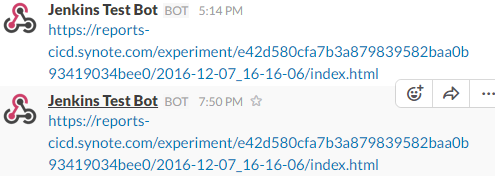
\includegraphics[width=0.78\textwidth]{slack-report-link.png}
  	\caption{Slack report link}
 	\label{fig:slack-report-link}
\end{figure}

\section{Usefulness of CI}
\label{sec:usefulness-of-ci}

\chapter{Further Work}
\label{chap:further-work}

% Lack of references due to the assumption that everything here has been touched upon within previous sections

Our interactions with the Synote code base have given us the opportunity to discover its existing strengths and weaknesses, as well as those introduced through our development. Existing weaknesses mostly correspond to the methodology for server side testing whereas the weaknesses we have introduced stem from learning technologies on the fly. With the knowledge we have ascertained at this point, we would propose several enhancements to Synote's design which we shall discuss as future work.\\ 

\subsection{Server Side Testing}
\label{subsec:server-side-testing}

Firstly, we believe that performing integration tests on \texttt{controllers} to test for situations that should be handled by \texttt{policies} is not desirable. The test shown in \textbf{Listing \ref{lst:creditcontroller-test-file}} is intending to check that the user requesting to view credits is himself the credit owner; an action that is performed in a \texttt{policy} named \texttt{canListCreditHistory.js}, not the \texttt{controller}.\\

Our solution is two fold. Firstly, the \texttt{policy} file should be unit tested using mocking and spying techniques. Secondly, the controller actions should be integration tested using dependency injection with a fake database. An example of our suggested \texttt{policy} testing convention is shown in \textbf{Listing \ref{lst:can-list-credit-test}} and demonstrates how the same test (with \texttt{admin} rule extension) can be written using a mocked request stub and a Sinon spy. This approach has the added benefit of running much faster than an \texttt{HTTP} request.  

\begin{listing}[H]
\begin{minted}[xleftmargin=\parindent, linenos, breaklines, breakanywhere, bgcolor=lightgray, fontsize=\small]{js}
it('should not view credit if not credit owner himself', function (done) {
      var user = testdata.getUserByEmail('yl2@ecs.soton.ac.uk');
      var anotheruser = testdata.getUserByEmail('mw@ecs.soton.ac.uk');
      var access_token = testdata.getUserTokenById(anotheruser.id);
      var c;
      Credit.findOne({owner: user.id}).then(function (credit) {
          c = credit;
          return request(sails.hooks.http.app)
              .get('/credit/' + credit.id)
              .set('Authorization', "Bearer " + access_token)
              .expect(403);
      }).then(function (res) {
          done();
      }).catch(done);
});
\end{minted}
\captionof{listing}{\texttt{CreditController.test.js} snippet}
\label{lst:creditcontroller-test-file}
\end{listing}

\begin{listing}[H]
\begin{minted}[xleftmargin=\parindent, linenos, breaklines, breakanywhere, bgcolor=lightgray, fontsize=\small]{js}
    var req, res, cb;

    beforeEach(function (done) {
        req = {
            user_profile: {
                id: '',
                role: ''
            },
            user: {sub: ''}
        };
        res = {};
        cb = sinon.spy();
        done();
    });

    it('If bearer does not match user and not admin, it is forbidden', function (done) {
        req.method = 'GET';
        req.user_profile.id = 'fakeid';
        req.user.sub = 'not matching fakeid';
        req.user.admin = 'not admin';
        res.forbidden = sinon.spy();

        canListCreditHitory(req, res, cb);

        expect(res.forbidden).called;
        expect(cb).not.called;
        done();
    });
\end{minted}
\captionof{listing}{\texttt{canListCreditHistory.test.js} snippet}
\label{lst:can-list-credit-test}
\end{listing}

\subsection{Auto Generated Page Objects}
\label{subsec:auto-generated-page-objects}

We envisioned an extension of our E2E testing framework to auto-generate page object files, but sadly it did not fall into the required feature set. The foundations for this enhancement exist in the form of our HTML ID convention such that a script could be produced to parse an HTML file and generate a page object skeleton based on element IDs. Automatic generation of required test framework skeleton files is also not limited to page objects. Partial templates for feature files and step files could also be generated as part of the envisioned script.\\    

\subsection{E2E Test Reporting}
\label{subsec:e2e-test-reporting}

At present, the E2E testing framework is responsible for generating a folder hierarchy  in which to save a test report based on: the latest Synote commit hash, current deployment and the date-time at which the test suite ran. At an earlier stage the framework was also responsible for posting a link to the generated report on Slack, but we believe the framework should not be responsible for either of these actions and consequently we have moved Slack posting tasks to the Jenkins CI script. The task of separating out the folder hierarchy generation still exists and is recommended as a future task.\\

\subsection{Ghost Inspector}
\label{subsec:ghost-inspector}

Our testing methodology contains a statement: \textit{If a component cannot be tested using our framework, it is considered a bug and should be changed}. In the case of Toastr alerts we adhered to this statement and developed an alternative alerts system. However another component, \texttt{cg-busy}, could also not be tested reliably. This component's use in Synote is desirable and consequently we implemented a test using Ghost Inspector to resolve the testing issue. Including Ghost Inspector in our E2E testing framework would be a fruitful future task resolving the need to compromise on component use.\\ 

\subsection{Testing Controller}
\label{subsec:testing-controller}



\subsection{Server Side Design}
\label{subsec:server-side-design}
\chapter{Conclusion}
\label{chap:conclusion}

\nocite{*}

%% bibliography
\addcontentsline{toc}{chapter}{Bibliography}
\bibliography{references}

%% appendix
\appendix
\chapter{Client Sign-off}
\label{appendix:client-sign-off}

\begin{figure}[!hbt]
  	\centering
 	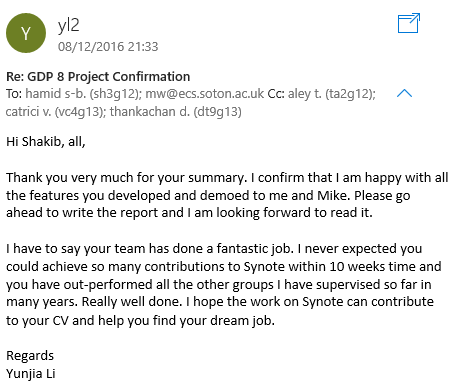
\includegraphics[width=\textwidth]{confirmation-email.png}
 	\caption{Client Sign off section}
\end{figure}
\chapter{Team Member Contribution}
\label{appendix:team-member-contribution}

\section{Shakib Contribution}
\label{sec:shakib-contribution}

\textbf{Supervisor Meeting} : All but 2 - Job interviews
\newline
\textbf{Amount of Work} : 35 Hours a week.
\newline
\textbf{Contribution} :

\begin{itemize}
 \item 20\% of the Synote server code for payment feature - refactoring policies, controllers, services
 \begin{itemize}
  \item Wrote the first version of server code with Tom
  \item Refactored the code again to implement with promises
 \end{itemize}
 \item 20\% of the E2E tests for Synote server code for
  payment feature.
 \begin{itemize}
  \item Test the REST API endpoints for the payment system
 \end{itemize}
 \item 20\% of the front end code for payment feature
 \begin{itemize}
  \item Refactor the controllers and the services multiple times
 \end{itemize}
 \item 60\% of the test framework code - pages, supports, deployment, structures
 \begin{itemize}
  \item Build the methodology of the test framework
  \item Implement the pages, reusable methods in support and reusable steps
  \item Implement the deployment definition
  \item Built the reporting website and the reporting structure to contain git commit hash, deployment and date (the latter with Tom)
  \item Wrote the readme.md or user guide for test framework
 \end{itemize}
 \item 25\% of the e2e test cases for the payment feature
 \begin{itemize}
  \item Write the first few test cases.
 \end{itemize}
 \item 60\% of the CI set up for Synote on experiment deployment.
 \begin{itemize}
  \item Install Jenkins on remote server, create user permissions and setup reverse proxy server
  \item Made the e2e tests runnable on remote servers (without a display) by using x-server (Xvfb), upgrading the deployment server (after estimating the ram and cpu requirements)
  \item Prepare Synote deployment with correct Linux permissions with Tom
  \item Write the Synote deployment automation script with Tom
 \end{itemize}
 \item 80\% of the contribution.md for Synote from our team
 \begin{itemize}
  \item QA process
  \item CI-CD
  \item Test case coverage
  \item Test case structure
 \end{itemize}
 \item Planning time, priorities for work
 \begin{itemize}
  \item Arrange weekly meetings with team and supervisor
  \item Guide the team discussions during weekly meetings
  \item Making sure team members are up to date with their other coursework
 \end{itemize}
 \item Code merges, deployments
 \begin{itemize}
  \item Make the code submission convention for the team
  \item Make weekly code pull requests
 \end{itemize}
 \item Research on Protractor, Sails, Angular, JavaScript
\end{itemize} 
\chapter{Team Collaboration}
\label{appendix:team-collaboration}

\begin{figure}[!hbt]
  	\centering
 	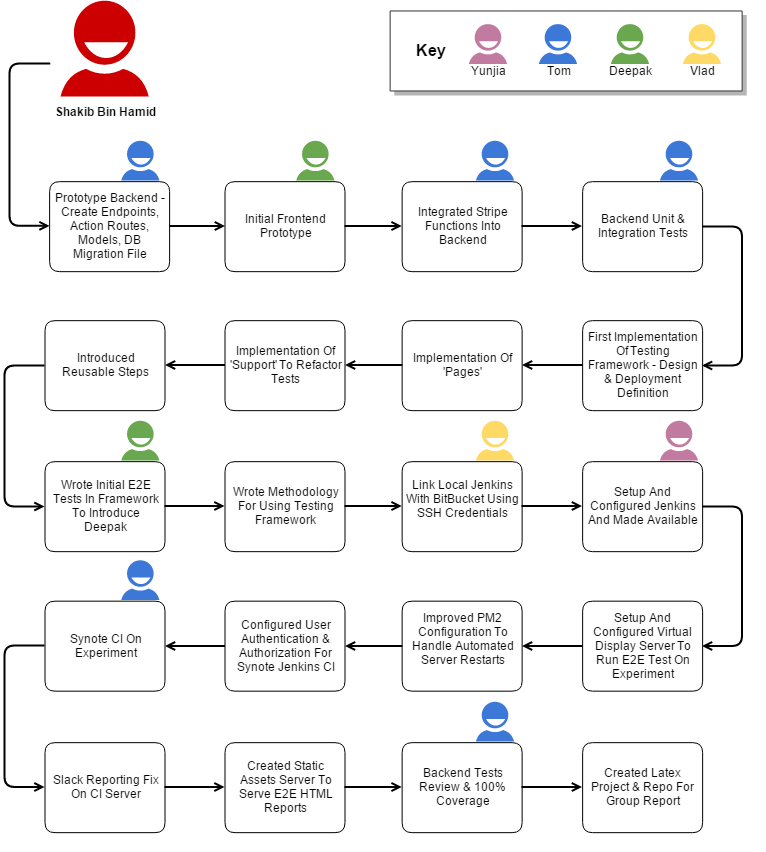
\includegraphics[width=1\textwidth]{shakib.png}
  	\caption{Shakib Bin Hamid - Workflow \& Collaboration Diagram}
 	\label{fig:shakib-collaboration}
\end{figure}

\begin{figure}[!hbt]
  	\centering
 	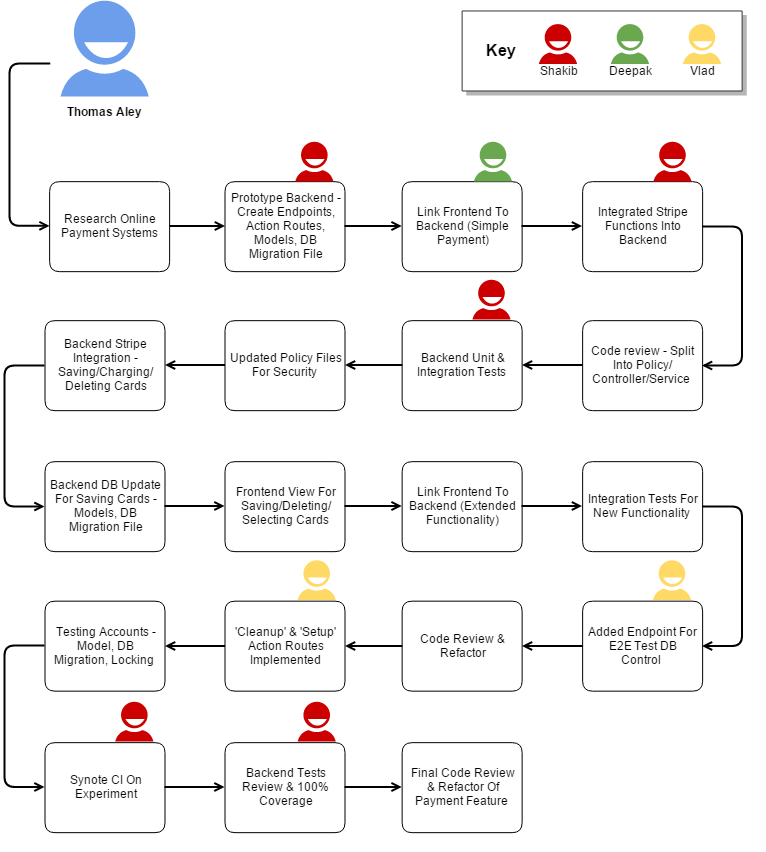
\includegraphics[width=1\textwidth]{tom.png}
  	\caption{Thomas Aley - Workflow \& Collaboration Diagram}
 	\label{fig:tom-collaboration}
\end{figure}

\begin{figure}[!hbt]
  	\centering
 	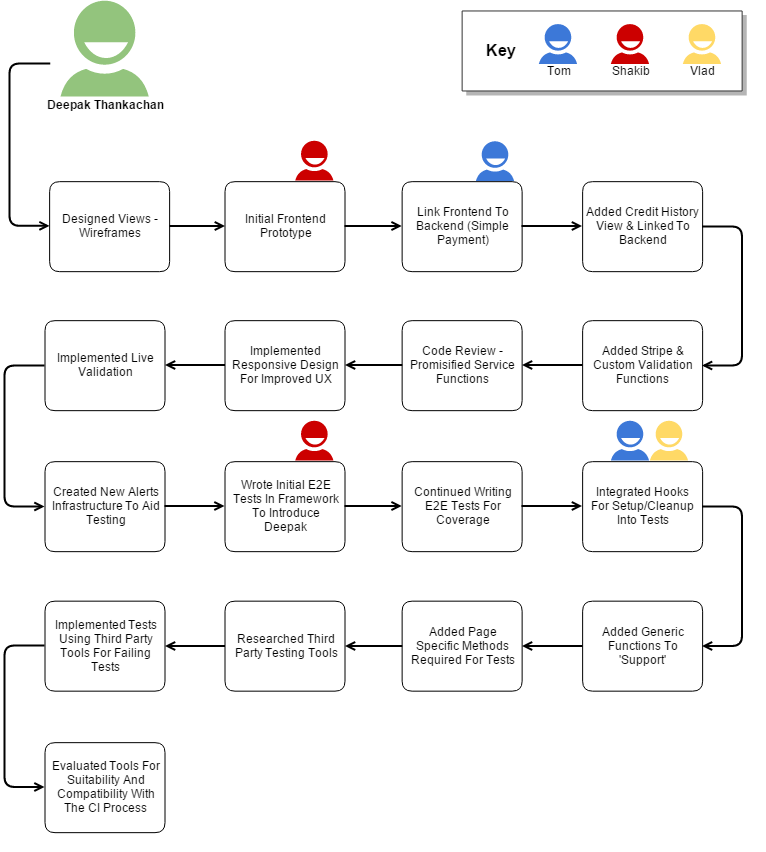
\includegraphics[width=1\textwidth]{deepak.png}
  	\caption{Deepak Thankachan - Workflow \& Collaboration Diagram}
 	\label{fig:deepak-collaboration}
\end{figure}

\begin{figure}[!hbt]
  	\centering
 	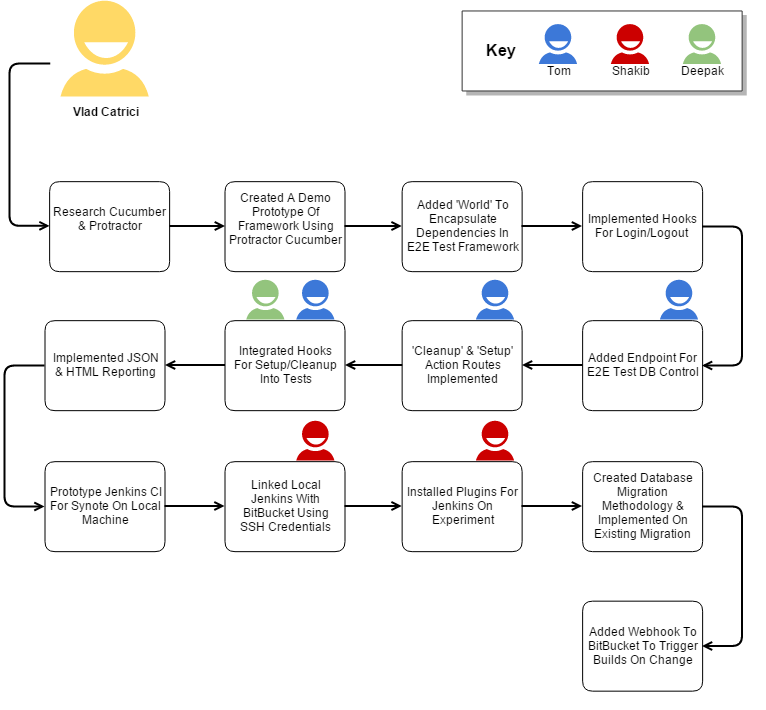
\includegraphics[width=1\textwidth]{vlad.png}
  	\caption{Vlad Catrici - Workflow \& Collaboration Diagram}
 	\label{fig:vlad-collaboration}
\end{figure}

\chapter{Code commits}
\label{appendix:code-commits}

\begin{figure}[!hbt]
  	\centering
 	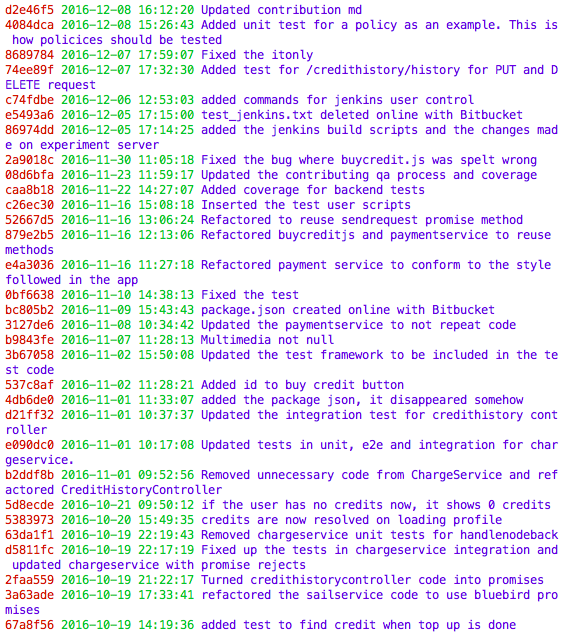
\includegraphics[width=1\textwidth]{synote-shak-1.png}
\end{figure}

\ContinuedFloat

\begin{figure}[!hbt]
  	\centering
 	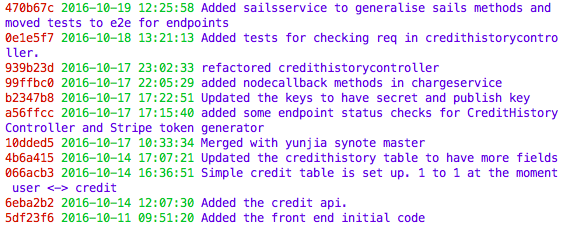
\includegraphics[width=1\textwidth]{synote-shak-2.png}
  	\caption{Shakib's Synote Commits}
 	\label{fig:shakib-synote-commits}
\end{figure}

\begin{figure}[!hbt]
  	\centering
 	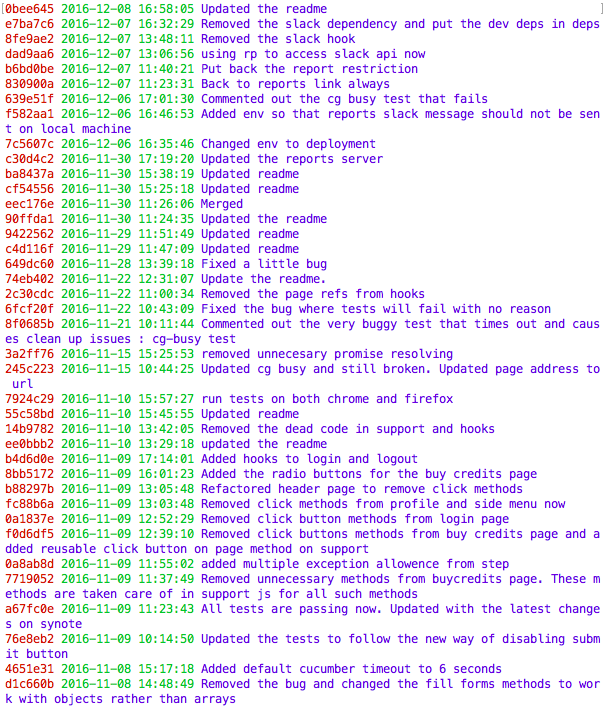
\includegraphics[width=1\textwidth]{test-shakib-1.png}
\end{figure}

\ContinuedFloat

\begin{figure}[!hbt]
  	\centering
 	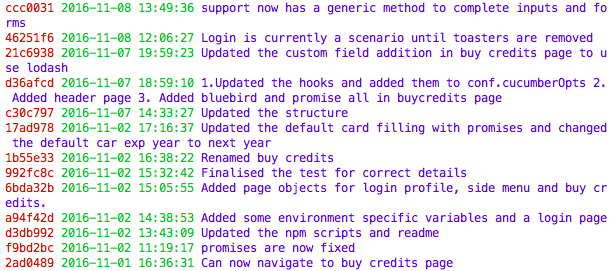
\includegraphics[width=1\textwidth]{test-shakib-2.png}
  	\caption{Shakib's Testing Framework Commits}
 	\label{fig:shakib-testing-commits}
\end{figure}

\begin{figure}[!hbt]
  	\centering
 	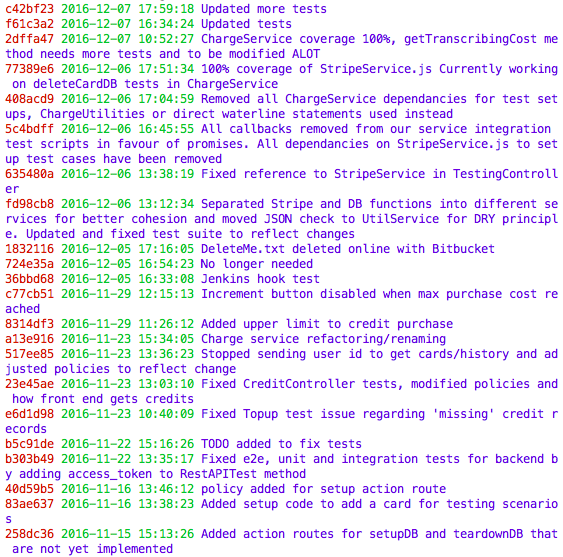
\includegraphics[width=1\textwidth]{synote-tom-1.png}
\end{figure}

\ContinuedFloat

\begin{figure}[!hbt]
  	\centering
 	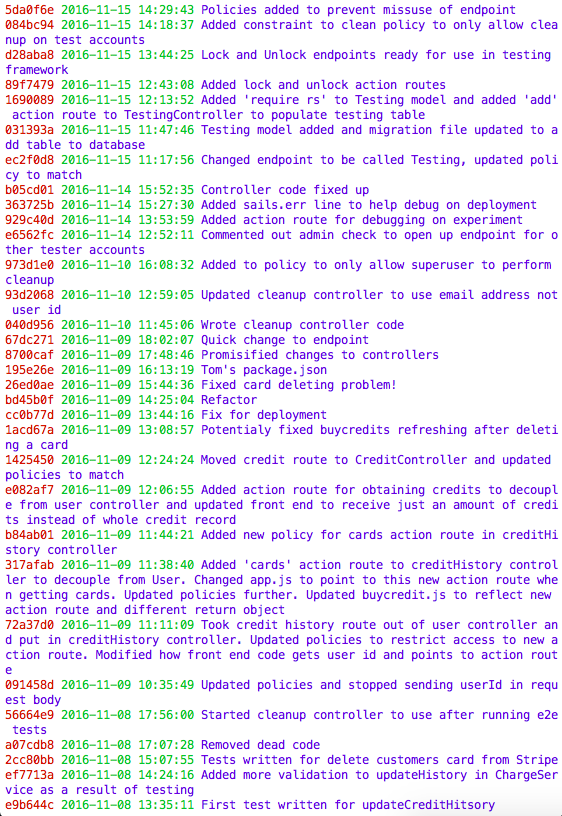
\includegraphics[width=1\textwidth]{synote-tom-2.png}
\end{figure}

\ContinuedFloat

\begin{figure}[!hbt]
  	\centering
 	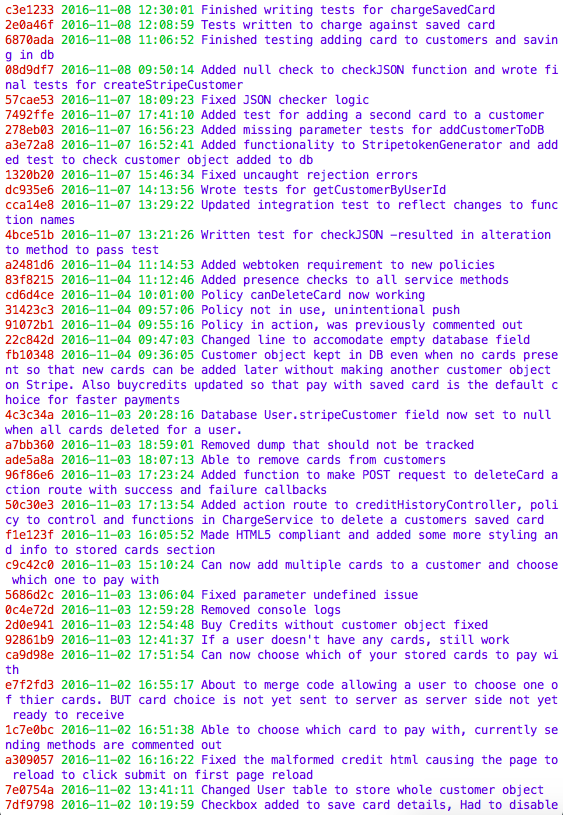
\includegraphics[width=1\textwidth]{synote-tom-3.png}
\end{figure}

\ContinuedFloat

\begin{figure}[!hbt]
  	\centering
 	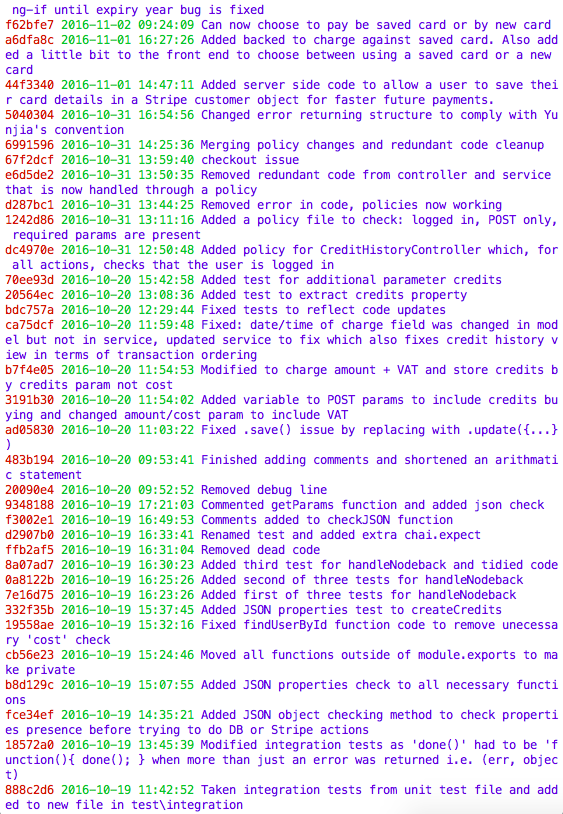
\includegraphics[width=1\textwidth]{synote-tom-4.png}
\end{figure}

\ContinuedFloat

\begin{figure}[!hbt]
  	\centering
 	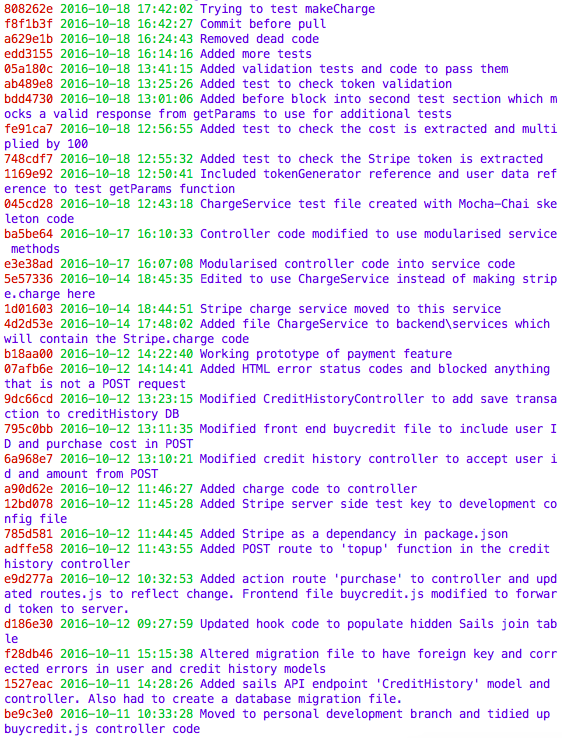
\includegraphics[width=1\textwidth]{synote-tom-5.png}
  	\caption{Tom's Synote Commits}
 	\label{fig:tom-synote-commits}
\end{figure}

\begin{figure}[!hbt]
  	\centering
 	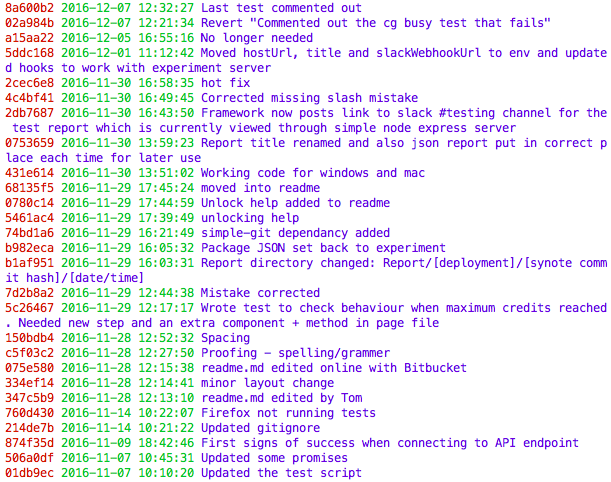
\includegraphics[width=1\textwidth]{test-tom-1.png}
  	\caption{Tom's Testing Framework Commits}
 	\label{fig:tom-testing-commits}
\end{figure}

\begin{figure}[!hbt]
  	\centering
 	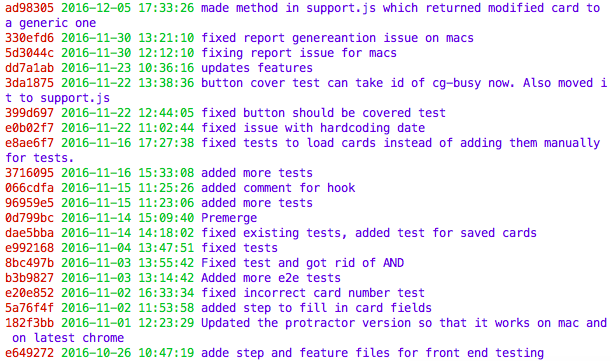
\includegraphics[width=1\textwidth]{test-deepak-1.png}
  	\caption{Deepak's Testing Framework Commits}
 	\label{fig:deepak-testing-commits}
\end{figure}

\begin{figure}[!hbt]
  	\centering
 	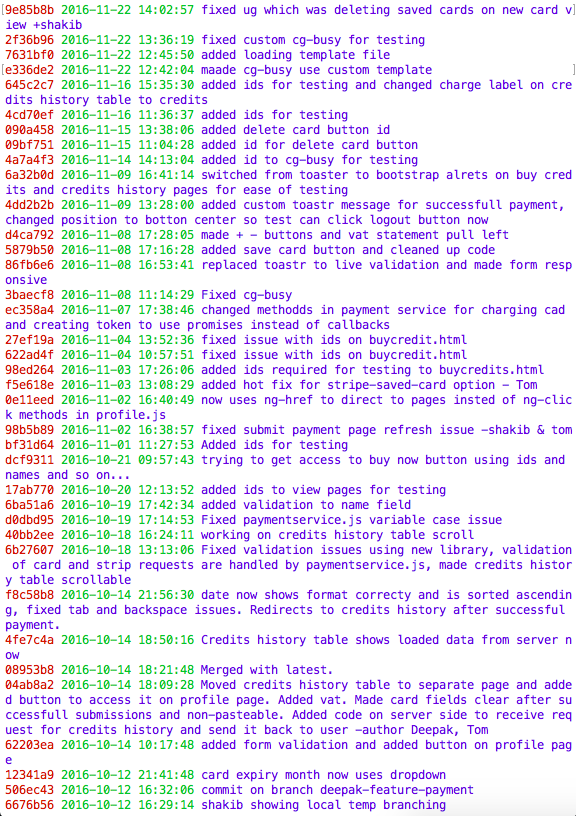
\includegraphics[width=1\textwidth]{synote-deepak-1.png}
  	\caption{Deepak's Synote Commits}
 	\label{fig:deepak-synote-commits}
\end{figure}

\begin{figure}[!hbt]
  	\centering
 	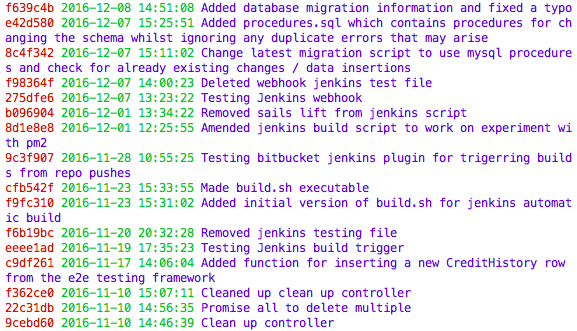
\includegraphics[width=1\textwidth]{synote-vlad-1.png}
  	\caption{Vlad's Synote Commits}
 	\label{fig:vlad-synote-commits}
\end{figure}

\begin{figure}[!hbt]
  	\centering
 	\includegraphics[width=1\textwidth]{test-vlad-1.png}
  	\caption{Vlad's Testing Framework Commits}
 	\label{fig:vlad-testing-commits}
\end{figure}
\chapter{Server Test Cases}
\label{appendix:server-test-cases}

\begin{figure}[!hbt]
  	\centering
 	\includegraphics[width=1\textwidth]{chargeservice-tests.png}
  	\caption{\texttt{ChargeService.js} Test Cases}
 	\label{fig:chargeservice-tests}
\end{figure}

\begin{figure}[!hbt]
  	\centering
 	\includegraphics[width=1\textwidth]{stripeservice-tests.png}
  	\caption{\texttt{StripeService.js} Test Cases}
 	\label{fig:stripeservice-tests}
\end{figure}

\begin{figure}[!hbt]
  	\centering
 	\includegraphics[width=1\textwidth]{remaining-tests.png}
  	\caption{Additional Test Cases}
 	\label{fig:additional-tests}
\end{figure}
\chapter{E2E Testing}
\label{appendix:e2e-testing}

\begin{figure}[!hbt]
  	\centering
 	\includegraphics[width=1\textwidth]{html-report.png}
  	\caption{HTML Reporting Screenshot}
 	\label{fig:html-reporting}
\end{figure}

%E2E Test Parts
\begin{figure}[!hbt]\ContinuedFloat
  	\centering
 	\includegraphics[width=1\textwidth]{e2e-test-part1.png}
\end{figure}

\begin{figure}[!hbt]\ContinuedFloat
  	\centering
	\includegraphics[width=1\textwidth]{e2e-test-part2.png}
\end{figure}

\begin{figure}[!hbt]\ContinuedFloat
  	\centering
	\includegraphics[width=1\textwidth]{e2e-test-part3.png}
\end{figure}

\begin{figure}[!hbt]
  	\centering
	\includegraphics[width=1\textwidth]{e2e-test-part4.png}
  	\caption{E2E Test Cases}
 	\label{fig:e2e-test-cases}
\end{figure}
%
\chapter{Gantt Charts}
\label{appendix:gantt-charts}

\pagebreak

\begin{sidewaysfigure}
    \centering
    \includegraphics[width=\linewidth]{gantt.pdf}
    \caption{Gantt Chart Latest and Initial}
    \label{fig:gantt-chart}
\end{sidewaysfigure}
\chapter{Payment Feature Screenshots}
\label{appendix:payment-feature-screenshots}

\begin{figure}[!hbt]
    \centering
  \includegraphics[width=0.5\textwidth]{screenshot-payment-form.png}
    \caption{Payment Form View}
  \label{fig:payment-form-screenshot}
\end{figure}

\begin{figure}[!hbt]
    \centering
  \includegraphics[width=0.7\textwidth]{screenshot-profile-page.png}
    \caption{Profile Page View}
  \label{fig:profile-screenshot}
\end{figure}

\begin{figure}[!hbt]
    \centering
  \includegraphics[width=0.7\textwidth]{screenshot-credit-history.png}
    \caption{Credits History View}
  \label{fig:credits-history-screenshot}
\end{figure}

\begin{figure}[!hbt]
    \centering
  \includegraphics[width=0.6\textwidth]{screenshot-saved-card-form.png}
    \caption{Saved Card Payment Form View}
  \label{fig:saved-cards-form-screenshot}
\end{figure}

\chapter{Report Contribution}
\label{appendix:report-contribution}

The contribution on the sections also include the subsections. Each team member wrote ~4500 words. They also reviewed and verified the whole report multiple times, aside from the following contribution.

\begin{longtable}{ |p{3cm}|p{10.4cm}|}

 \hline
 	\multicolumn{2}{|c|}{Report Contribution} \\
  \hline
    \multicolumn{1}{|c|}{Team Member} &
  	\multicolumn{1}{|c|}{Report Contribution} \\
  \hline
 	 Shakib-Bin Hamid & Chapter 1, 2, 6 (except Section 6.1.2 and 6.3.1) \\
   \hline
   Thomas Aley & Section 3.1.4, 3.2, 4.1, 4.2, Chapter 7 \\
   \hline
   Deepak Thankachan & Section 3.2 - 3.4, 4.3, 5.3 \\
  \hline
  Vlad Catrici & Section 3.5 - 3.7, 5.1, 5.2, 6.1.2, 6.3.1, Chapter 8\\
  \hline
  \caption{Report Contribution}
  \label{tab:report-contribution}
\end{longtable}


\end{document}
